%&preformat-synopsis
\RequirePackage[l2tabu,orthodox]{nag} % Раскомментировав, можно в логе получать рекомендации относительно правильного использования пакетов и предупреждения об устаревших и нерекомендуемых пакетах

% Откомментируйте, чтобы отключить генерацию закладок в pdf
% \PassOptionsToPackage{bookmarks=false}{hyperref}
\documentclass[a5paper,10pt,twoside,openany,article]{memoir} %,draft

%%%%%%%%%%%%%%%%%%%%%%%%%%%%%%%%%%%%%%%%%%%%%%%%%%%%%%%%%%%%%%%%%%%%%%%%%%%%%%%%
%%%% Файл упрощённых настроек шаблона, общих для диссертации и автореферата %%%%
%%%%%%%%%%%%%%%%%%%%%%%%%%%%%%%%%%%%%%%%%%%%%%%%%%%%%%%%%%%%%%%%%%%%%%%%%%%%%%%%

%%% Режим черновика %%%
\makeatletter
\@ifundefined{c@draft}{
  \newcounter{draft}
  \setcounter{draft}{0}  % 0 --- чистовик (максимальное соблюдение ГОСТ)
                         % 1 --- черновик (отклонения от ГОСТ, но быстрая
                         %       сборка итоговых PDF)
}{}
\makeatother

%%% Пометки в тексте %%%
\makeatletter
\@ifundefined{c@showmarkup}{
  \newcounter{showmarkup}
  \setcounter{showmarkup}{0}  % 0 --- скрыть пометки
                              % 1 --- показывать пометки
}{}
\makeatother

%%% Диссертация на английском %%%
\makeatletter
\@ifundefined{c@englishthesis}{
  \newcounter{englishthesis}
  \setcounter{englishthesis}{1}  % 0 --- диссертация на русском
                                 % 1 --- диссертация на английском; влияет 
                                 %       на подписи к рисункам и прочее
}{}
\makeatother

%%% Использование в pdflatex шрифтов не по-умолчанию %%%
\makeatletter
\@ifundefined{c@usealtfont}{
  \newcounter{usealtfont}
  \setcounter{usealtfont}{1}    % 0 --- шрифты на базе Computer Modern
                                % 1 --- использовать пакет pscyr, при его
                                %       наличии
                                % 2 --- использовать пакет XCharter, при наличии
                                %       подходящей версии
}{}
\makeatother

%%% Использование в xelatex и lualatex семейств шрифтов %%%
\makeatletter
\@ifundefined{c@fontfamily}{
  \newcounter{fontfamily}
  \setcounter{fontfamily}{1}  % 0 --- CMU семейство. Используется как fallback;
                              % 1 --- Шрифты от MS (Times New Roman и компания)
                              % 2 --- Семейство Liberation
}{}
\makeatother

%%% Библиография %%%
\makeatletter
\@ifundefined{c@bibliosel}{
  \newcounter{bibliosel}
  \setcounter{bibliosel}{1}   % 0 --- встроенная реализация с загрузкой файла
                              %       через движок bibtex8;
                              % 1 --- реализация пакетом biblatex через движок
                              %       biber
}{}
\makeatother

%%% Вывод типов ссылок в библиографии %%%
\makeatletter
\@ifundefined{c@mediadisplay}{
  \newcounter{mediadisplay}
  \setcounter{mediadisplay}{3}   % 0 --- не делать ничего; надписи [Текст] и
                                 %       [Эл. ресурс] будут выводиться только в ссылках с
                                 %       заполненным полем `media`;
                                 % 1 --- автоматически добавлять надпись [Текст] к ссылкам с
                                 %       незаполненным полем `media`; таким образом, у всех
                                 %       источников будет указан тип, что соответствует
                                 %       требованиям ГОСТ
                                 % 2 --- автоматически удалять надписи [Текст], [Эл. Ресурс] и др.;
                                 %       не соответствует ГОСТ
                                 % 3 --- автоматически удалять надпись [Текст];
                                 %       не соответствует ГОСТ
                                 % 4 --- автоматически удалять надпись [Эл. Ресурс];
                                 %       не соответствует ГОСТ
}{}
\makeatother

%%% Предкомпиляция tikz рисунков для ускорения работы %%%
\makeatletter
\@ifundefined{c@imgprecompile}{
  \newcounter{imgprecompile}
  \setcounter{imgprecompile}{0}   % 0 --- без предкомпиляции;
                                  % 1 --- пользоваться предварительно
                                  %       скомпилированными pdf вместо генерации
                                  %       заново из tikz
}{}
\makeatother
          % общие настройки шаблона
%%% Проверка используемого TeX-движка %%%
\newif\ifxetexorluatex   % определяем новый условный оператор (http://tex.stackexchange.com/a/47579)
\ifxetex
    \xetexorluatextrue
\else
    \ifluatex
        \xetexorluatextrue
    \else
        \xetexorluatexfalse
    \fi
\fi

\newif\ifsynopsis           % Условие, проверяющее, что документ --- автореферат

\usepackage{etoolbox}[2015/08/02]   % Для продвинутой проверки разных условий
\providebool{presentation}

\usepackage{comment}    % Позволяет убирать блоки текста (добавляет
                        % окружение comment и команду \excludecomment)

%%% Поля и разметка страницы %%%
\usepackage{pdflscape}  % Для включения альбомных страниц
\usepackage{geometry}   % Для последующего задания полей

%%% Математические пакеты %%%
\usepackage{amsthm,amsmath,amscd}   % Математические дополнения от AMS
\usepackage{amsfonts,amssymb}       % Математические дополнения от AMS
\usepackage{mathtools}              % Добавляет окружение multlined
\usepackage{xfrac}                  % Красивые дроби
\usepackage[
    locale = DE,
    list-separator       = {;\,},
    list-final-separator = {;\,},
    list-pair-separator  = {;\,},
    list-units           = single,
    range-units          = single,
    range-phrase={\text{\ensuremath{-}}},
    % quotient-mode        = fraction, % красивые дроби могут не соответствовать ГОСТ
    fraction-function    = \sfrac,
    separate-uncertainty,
    ]{siunitx}[=v2]                 % Размерности SI
\sisetup{inter-unit-product = \ensuremath{{}\cdot{}}}


% Кириллица в нумерации subequations
% Для правильной работы требуется выполнение сразу после загрузки пакетов
\ifnumequal{\value{englishthesis}}{0}{
    \patchcmd{\subequations}{\def\theequation{\theparentequation\alph{equation}}}
    {\def\theequation{\theparentequation\asbuk{equation}}}
    {\typeout{subequations patched}}{\typeout{subequations not patched}}
}{}
% \patchcmd{\subequations}{\def\theequation{\theparentequation\alph{equation}}}
% {\def\theequation{\theparentequation\asbuk{equation}}}
% {\typeout{subequations patched}}{\typeout{subequations not patched}}

%%%% Установки для размера шрифта 14 pt %%%%
%% Формирование переменных и констант для сравнения (один раз для всех подключаемых файлов)%%
%% должно располагаться до вызова пакета fontspec или polyglossia, потому что они сбивают его работу
\newlength{\curtextsize}
\newlength{\bigtextsize}
\setlength{\bigtextsize}{13.9pt}

\makeatletter
%\show\f@size    % неплохо для отслеживания, но вызывает стопорение процесса,
                 % если документ компилируется без команды  -interaction=nonstopmode
\setlength{\curtextsize}{\f@size pt}
\makeatother

%%% Кодировки и шрифты %%%
\ifxetexorluatex
    \ifpresentation
        \providecommand*\autodot{} % quick fix for polyglossia 1.50
    \fi
    \PassOptionsToPackage{no-math}{fontspec}    % https://tex.stackexchange.com/a/26295/104425
    \usepackage{polyglossia}[2014/05/21]        % Поддержка многоязычности
                                        % (fontspec подгружается автоматически)
\else
   %%% Решение проблемы копирования текста в буфер кракозябрами
    \ifnumequal{\value{usealtfont}}{0}{}{
        \input glyphtounicode.tex
        \input glyphtounicode-cmr.tex %from pdfx package
        \pdfgentounicode=1
    }
    \usepackage{cmap}   % Улучшенный поиск русских слов в полученном pdf-файле
    \ifnumequal{\value{usealtfont}}{2}{}{
        \defaulthyphenchar=127  % Если стоит до fontenc, то переносы
                                % не впишутся в выделяемый текст при
                                % копировании его в буфер обмена
    }
    \usepackage{textcomp}
    \usepackage[T1,T2A]{fontenc}                    % Поддержка русских букв
    \ifnumequal{\value{usealtfont}}{1}{% Используется pscyr, при наличии
        \IfFileExists{pscyr.sty}{\usepackage{pscyr}}{}  % Подключение pscyr
    }{}
    \usepackage[utf8]{inputenc}[2014/04/30]         % Кодировка utf8
    \ifnumequal{\value{englishthesis}}{0}{
        \usepackage[english, russian]{babel}[2014/03/24]% Языки: русский, английский
    }{
        \usepackage[english]{babel}[2014/03/24]% Языки: английский
    }



    \makeatletter\AtBeginDocument{\let\@elt\relax}\makeatother % babel 3.40 fix
    \ifnumequal{\value{usealtfont}}{2}{
        % http://dxdy.ru/post1238763.html#p1238763
        \usepackage[scaled=0.914]{XCharter}[2017/12/19] % Подключение русифицированных шрифтов XCharter
        \usepackage[charter, vvarbb, scaled=1.048]{newtxmath}[2017/12/14]
        \ifpresentation
        \else
            \setDisplayskipStretch{-0.078}
        \fi
    }{}
\fi

%%% Оформление абзацев %%%
\ifpresentation
\else
    \indentafterchapter     % Красная строка после заголовков типа chapter
    \usepackage{indentfirst}
\fi

%%% Цвета %%%
\ifpresentation
\else
    \usepackage[dvipsnames, table, hyperref]{xcolor} % Совместимо с tikz
\fi

%%% Таблицы %%%
\usepackage{longtable,ltcaption} % Длинные таблицы
\usepackage{multirow,makecell}   % Улучшенное форматирование таблиц
\usepackage{tabu, tabulary}      % таблицы с автоматически подбирающейся
                                 % шириной столбцов (tabu обязательно
                                 % до hyperref вызывать)
\makeatletter
%https://github.com/tabu-issues-for-future-maintainer/tabu/issues/26
\@ifpackagelater{longtable}{2020/02/07}{
\def\tabuendlongtrial{%
    \LT@echunk  \global\setbox\LT@gbox \hbox{\unhbox\LT@gbox}\kern\wd\LT@gbox
                \LT@get@widths
}%
}{}
\makeatother

\usepackage{threeparttable}      % автоматический подгон ширины подписи таблицы

%%% Общее форматирование
\usepackage{soulutf8}% Поддержка переносоустойчивых подчёркиваний и зачёркиваний
\usepackage{icomma}  % Запятая в десятичных дробях

%%% Оптимизация расстановки переносов и длины последней строки абзаца
\IfFileExists{impnattypo.sty}{% проверка установленности пакета impnattypo
    \ifluatex
        \ifnumequal{\value{draft}}{1}{% Черновик
            \usepackage[hyphenation, lastparline, nosingleletter, homeoarchy,
            rivers, draft]{impnattypo}
        }{% Чистовик
            \usepackage[hyphenation, lastparline, nosingleletter]{impnattypo}
        }
    \else
        \usepackage[hyphenation, lastparline]{impnattypo}
    \fi
}{}

%% Векторная графика

\usepackage{tikz}                   % Продвинутый пакет векторной графики
\usetikzlibrary{chains}             % Для примера tikz рисунка
\usetikzlibrary{shapes.geometric}   % Для примера tikz рисунка
\usetikzlibrary{shapes.symbols}     % Для примера tikz рисунка
\usetikzlibrary{arrows}             % Для примера tikz рисунка

%%% Гиперссылки %%%
\ifxetexorluatex
    \let\CYRDZE\relax
\fi
\usepackage{hyperref}[2012/11/06]

%%% Изображения %%%
\usepackage{graphicx}[2014/04/25]   % Подключаем пакет работы с графикой
\usepackage{caption}                % Подписи рисунков и таблиц
\usepackage{subcaption}             % Подписи подрисунков и подтаблиц
\usepackage{pdfpages}               % Добавление внешних pdf файлов

%%% Счётчики %%%
\usepackage{aliascnt}
\usepackage[figure,table]{totalcount}   % Счётчик рисунков и таблиц
\usepackage{totcount}   % Пакет создания счётчиков на основе последнего номера
                        % подсчитываемого элемента (может требовать дважды
                        % компилировать документ)
\usepackage{totpages}   % Счётчик страниц, совместимый с hyperref (ссылается
                        % на номер последней страницы). Желательно ставить
                        % последним пакетом в преамбуле

%%% Продвинутое управление групповыми ссылками (пока только формулами) %%%
\ifpresentation
\else
    \ifnumequal{\value{englishthesis}}{0}{
        \usepackage[russian]{cleveref} % cleveref имеет сложности со считыванием
    % языка из babel. Такое решение русификации вывода выбрано вместо
    % определения в documentclass из опасности что-то лишнее передать во все
    % остальные пакеты, включая библиографию.
    }{
        \usepackage{cleveref}
    }
    % Добавление возможности использования пробелов в \labelcref
    % https://tex.stackexchange.com/a/340502/104425
    \usepackage{kvsetkeys}
    \makeatletter
    \let\org@@cref\@cref
    \renewcommand*{\@cref}[2]{%
        \edef\process@me{%
            \noexpand\org@@cref{#1}{\zap@space#2 \@empty}%
        }\process@me
    }
    \makeatother
\fi

\usepackage{placeins} % для \FloatBarrier

\ifnumequal{\value{draft}}{1}{% Черновик
    \usepackage[firstpage]{draftwatermark}
    \SetWatermarkText{DRAFT}
    \SetWatermarkFontSize{14pt}
    \SetWatermarkScale{15}
    \SetWatermarkAngle{45}
}{}

%%% Цитата, не приводимая в автореферате:
% возможно, актуальна только для biblatex
%\newcommand{\citeinsynopsis}[1]{\ifsynopsis\else ~\cite{#1} \fi}

% если текущий процесс запущен библиотекой tikz-external, то прекомпиляция должна быть включена
\ifdefined\tikzexternalrealjob
    \setcounter{imgprecompile}{1}
\fi

\ifnumequal{\value{imgprecompile}}{1}{% Только если у нас включена предкомпиляция
    \usetikzlibrary{external}   % подключение возможности предкомпиляции
    \tikzexternalize[prefix=images/cache/,optimize command away=\includepdf] % activate! % здесь можно указать отдельную папку для скомпилированных файлов
    \ifxetex
        \tikzset{external/up to date check={diff}}
    \fi
}{}


\usepackage{physics}
\usepackage{bbm}
\usepackage{qcircuit}
\usepackage{tabularx}
\usepackage[export]{adjustbox}
\usepackage{oplotsymbl}
% \usepackage{color}       % Пакеты общие для диссертации и автореферата
\synopsistrue                 % Этот документ --- автореферат
\input{Synopsis/synpackages}  % Пакеты для автореферата
\input{Synopsis/userpackages} % Пакеты для специфических пользовательских задач

% Новые переменные, которые могут использоваться во всём проекте
% ГОСТ 7.0.11-2011
% 9.2 Оформление текста автореферата диссертации
% 9.2.1 Общая характеристика работы включает в себя следующие основные структурные
% элементы:
% актуальность темы исследования;
\newcommand{\actualityTXT}{Актуальность темы.}
% степень ее разработанности;
\newcommand{\progressTXT}{Степень разработанности темы.}
% цели и задачи;
\newcommand{\aimTXT}{Целью}
\newcommand{\tasksTXT}{задачи}
% научную новизну;
\newcommand{\noveltyTXT}{Научная новизна:}
% теоретическую и практическую значимость работы;
%\newcommand{\influenceTXT}{Теоретическая и практическая значимость}
% или чаще используют просто
\newcommand{\influenceTXT}{Практическая значимость}
% методологию и методы исследования;
\newcommand{\methodsTXT}{Методология и методы исследования.}
% положения, выносимые на защиту;
\newcommand{\defpositionsTXT}{Основные положения, выносимые на~защиту:}
% степень достоверности и апробацию результатов.
\newcommand{\reliabilityTXT}{Достоверность}
\newcommand{\probationTXT}{Апробация работы.}

\newcommand{\contributionTXT}{Личный вклад.}
\newcommand{\publicationsTXT}{Публикации.}


%%% Заголовки библиографии:

% для автореферата:
\newcommand{\bibtitleauthor}{Публикации автора по теме диссертации}
\newcommand{\bibtitleauthorEn}{Author's publications on the dissertation subject}


% для стиля библиографии `\insertbiblioauthorgrouped`
\newcommand{\bibtitleauthorvak}{В изданиях из списка ВАК РФ}
\newcommand{\bibtitleauthorscopus}{В изданиях, входящих в международную базу цитирования Scopus}
\newcommand{\bibtitleauthorwos}{В изданиях, входящих в международную базу цитирования Web of Science}
\newcommand{\bibtitleauthorother}{В прочих изданиях}
\newcommand{\bibtitleauthorconf}{В сборниках трудов конференций}
\newcommand{\bibtitleauthorpatent}{Зарегистрированные патенты}
\newcommand{\bibtitleauthorprogram}{Зарегистрированные программы для ЭВМ}

% для стиля библиографии `\insertbiblioauthorimportant`:
\newcommand{\bibtitleauthorimportant}{Наиболее значимые \protect\MakeLowercase\bibtitleauthor}

% для списка литературы в диссертации и списка чужих работ в автореферате:
\newcommand{\bibtitlefull}{Список литературы} % (ГОСТ Р 7.0.11-2011, 4)
\newcommand{\bibtitlefullEn}{Bibliography}



% Aliases for popular symbols
\newcommand{\mc}[1]{\mathcal{#1}}
\newcommand{\id}{\mathbbm{1}}
\newcommand{\rmi}{\mathrm{i}}
\newcommand{\placeholder}{\ast}

\DeclareMathOperator{\Var}{Var}

\tikzset{blank/.style={rectangle,inner sep=0pt,draw=none,fill=none,minimum
    size=0pt} }       % Новые переменные, которые могут использоваться во всём проекте
%%%%%%%%%%%%%%%%%%%%%%%%%%%%%%%%%%%%%%%%%%%%%%%%%%%%%%%
%%%% Файл упрощённых настроек шаблона автореферата %%%%
%%%%%%%%%%%%%%%%%%%%%%%%%%%%%%%%%%%%%%%%%%%%%%%%%%%%%%%

%%% Инициализирование переменных, не трогать!  %%%
\newcounter{showperssign}
\newcounter{showsecrsign}
\newcounter{showopplead}
%%%%%%%%%%%%%%%%%%%%%%%%%%%%%%%%%%%%%%%%%%%%%%%%%%%%%%%

%%% Список публикаций %%%
\makeatletter
\@ifundefined{c@usefootcite}{
  \newcounter{usefootcite}
  \setcounter{usefootcite}{0} % 0 --- два списка литературы;
                              % 1 --- список публикаций автора + цитирование
                              %       других работ в сносках
}{}
\makeatother

\makeatletter
\@ifundefined{c@bibgrouped}{
  \newcounter{bibgrouped}
  \setcounter{bibgrouped}{0}  % 0 --- единый список работ автора;
                              % 1 --- сгруппированные работы автора
}{}
\makeatother

%%% Область упрощённого управления оформлением %%%

%% Управление зазором между подрисуночной подписью и основным текстом %%
\setlength{\belowcaptionskip}{10pt plus 20pt minus 2pt}


%% Подпись таблиц %%

% смещение строк подписи после первой
\newcommand{\tabindent}{0cm}

% тип форматирования таблицы
% plain --- название и текст в одной строке
% split --- название и текст в разных строках
\newcommand{\tabformat}{plain}

%%% настройки форматирования таблицы `plain'

% выравнивание по центру подписи, состоящей из одной строки
% true  --- выравнивать
% false --- не выравнивать
\newcommand{\tabsinglecenter}{false}

% выравнивание подписи таблиц
% justified   --- выравнивать как обычный текст
% centering   --- выравнивать по центру
% centerlast  --- выравнивать по центру только последнюю строку
% centerfirst --- выравнивать по центру только первую строку
% raggedleft  --- выравнивать по правому краю
% raggedright --- выравнивать по левому краю
\newcommand{\tabjust}{justified}

% Разделитель записи «Таблица #» и названия таблицы
\newcommand{\tablabelsep}{~\cyrdash\ }

%%% настройки форматирования таблицы `split'

% положение названия таблицы
% \centering   --- выравнивать по центру
% \raggedleft  --- выравнивать по правому краю
% \raggedright --- выравнивать по левому краю
\newcommand{\splitformatlabel}{\raggedleft}

% положение текста подписи
% \centering   --- выравнивать по центру
% \raggedleft  --- выравнивать по правому краю
% \raggedright --- выравнивать по левому краю
\newcommand{\splitformattext}{\raggedright}

%% Подпись рисунков %%
%Разделитель записи «Рисунок #» и названия рисунка
\newcommand{\figlabelsep}{~\cyrdash\ }  % (ГОСТ 2.105, 4.3.1)
                                        % "--- здесь не работает

%Демонстрация подписи диссертанта на автореферате
\setcounter{showperssign}{0}  % 0 --- не показывать;
                              % 1 --- показывать
%Демонстрация подписи учёного секретаря на автореферате
\setcounter{showsecrsign}{0}  % 0 --- не показывать;
                              % 1 --- показывать
%Демонстрация информации об оппонентах и ведущей организации на автореферате
\setcounter{showopplead}{1}   % 0 --- не показывать;
                              % 1 --- показывать

%%% Цвета гиперссылок %%%
% Latex color definitions: http://latexcolor.com/
% \definecolor{linkcolor}{rgb}{0.9,0,0}
% \definecolor{citecolor}{rgb}{0,0.6,0}
% \definecolor{urlcolor}{rgb}{0,0,1}
\definecolor{linkcolor}{rgb}{0,0,0} %black
\definecolor{citecolor}{rgb}{0,0,0} %black
\definecolor{urlcolor}{rgb}{0,0,0} %black
        % Упрощённые настройки шаблона

%%% Основные сведения %%%
\newcommand{\thesisAuthorLastName}{Уваров}
\newcommand{\thesisAuthorOtherNames}{Алексей Викторович}
\newcommand{\thesisAuthorInitials}{А.\,В.}
\newcommand{\thesisAuthorLastNameEn}{Uvarov}
\newcommand{\thesisAuthorOtherNamesEn}{Alexey Viktorovich}
\newcommand{\thesisAuthorInitialsEn}{A.\,V.}

\newcommand{\thesisAuthor}             % Диссертация, ФИО автора
{%
    \texorpdfstring{% \texorpdfstring takes two arguments and uses the first for (La)TeX and the second for pdf
        \thesisAuthorLastName~\thesisAuthorOtherNames% так будет отображаться на титульном листе или в тексте, где будет использоваться переменная
    }{%
        \thesisAuthorLastName, \thesisAuthorOtherNames% эта запись для свойств pdf-файла. В таком виде, если pdf будет обработан программами для сбора библиографических сведений, будет правильно представлена фамилия.
    }
}
\newcommand{\thesisAuthorEn}             % Диссертация, ФИО автора
{%
    \texorpdfstring{% \texorpdfstring takes two arguments and uses the first for (La)TeX and the second for pdf
        \thesisAuthorLastNameEn~\thesisAuthorOtherNamesEn% так будет отображаться на титульном листе или в тексте, где будет использоваться переменная
    }{%
        \thesisAuthorLastNameEn, \thesisAuthorOtherNamesEn% эта запись для свойств pdf-файла. В таком виде, если pdf будет обработан программами для сбора библиографических сведений, будет правильно представлена фамилия.
    }
}

\newcommand{\thesisAuthorShort}        % Диссертация, ФИО автора инициалами
{\thesisAuthorInitials~\thesisAuthorLastName}
\newcommand{\thesisAuthorShortEn}        % Диссертация, ФИО автора инициалами
{\thesisAuthorInitialsEn~\thesisAuthorLastNameEn}

%\newcommand{\thesisUdk}                % Диссертация, УДК
%{\fixme{xxx.xxx}}
\newcommand{\thesisTitle}              % Диссертация, название
{Вариационные квантовые алгоритмы для решения задач минимизации локальных гамильтонианов}
\newcommand{\thesisTitleEn}              % Диссертация, название
{Variational quantum algorithms for local Hamiltonian problems}
\newcommand{\thesisSpecialtyNumber}    % Диссертация, специальность, номер
{1.3.3}
\newcommand{\thesisSpecialtyTitle}     % Диссертация, специальность, название (название взято с сайта ВАК для примера)
{Теоретическая физика}
\newcommand{\thesisSpecialtyTitleEn}     % Диссертация, специальность, название (название взято с сайта ВАК для примера)
{Theoretical physics}
%% \newcommand{\thesisSpecialtyTwoNumber} % Диссертация, вторая специальность, номер
%% {\fixme{XX.XX.XX}}
%% \newcommand{\thesisSpecialtyTwoTitle}  % Диссертация, вторая специальность, название
%% {\fixme{Теория и~методика физического воспитания, спортивной тренировки,
%% оздоровительной и~адаптивной физической культуры}}
\newcommand{\thesisDegree}             % Диссертация, ученая степень
{кандидата физико-математических наук}
\newcommand{\thesisDegreeEn}             % Диссертация, ученая степень
{Candidate of Physical and Mathematical Sciences}
\newcommand{\thesisDegreeShort}        % Диссертация, ученая степень, краткая запись
{канд.~физ.-мат.~наук}
\newcommand{\thesisDegreeShortEn}        % Диссертация, ученая степень, краткая запись
{cand.~of phys.-math.~sciences}
\newcommand{\thesisCity}               % Диссертация, город написания диссертации
{Москва}
\newcommand{\thesisCityEn}               % Диссертация, город написания диссертации
{Moscow}
\newcommand{\thesisYear}               % Диссертация, год написания диссертации
{2023}
\newcommand{\thesisOrganization}       % Диссертация, организация
{Автономная некоммерческая образовательная организация высшего профессионального образования <<Сколковский институт науки и технологий>>}
\newcommand{\thesisOrganizationEn}       % Диссертация, организация
{Autonomous Non-Profit Organization for Higher Education <<Skolkovo Institute of Science and Technology>>}
\newcommand{\thesisOrganizationShort}  % Диссертация, краткое название организации для доклада
{Сколтех}
\newcommand{\thesisOrganizationShortEn}  % Диссертация, краткое название организации для доклада
{Skoltech}

\newcommand{\thesisInOrganization}     % Диссертация, организация в предложном падеже: Работа выполнена в ...
{Автономной некоммерческой образовательной организации высшего профессионального образования <<Сколковский институт науки и технологий>>}

%% \newcommand{\supervisorDead}{}           % Рисовать рамку вокруг фамилии
\newcommand{\supervisorFio}              % Научный руководитель, ФИО
{Биамонте Джейкоб Дэниел }
\newcommand{\supervisorRegalia}          % Научный руководитель, регалии
{доктор физико-математических наук, профессор}
\newcommand{\supervisorFioShort}         % Научный руководитель, ФИО
{Дж.\,Д.~Биамонте}
\newcommand{\supervisorRegaliaShort}     % Научный руководитель, регалии
{д.~ф.-м.~н, проф.}

\newcommand{\supervisorFioEn}              % Научный руководитель, ФИО
{Biamonte Jacob Daniel }
\newcommand{\supervisorRegaliaEn}          % Научный руководитель, регалии
{Doctor of Physical and Mathematical Sciences, Professor}
\newcommand{\supervisorFioShortEn}         % Научный руководитель, ФИО
{\fixme{J.\,D.~Biamonte}}
\newcommand{\supervisorRegaliaShortEn}     % Научный руководитель, регалии
{\fixme{D.Sc., Prof}}

%% \newcommand{\supervisorTwoDead}{}        % Рисовать рамку вокруг фамилии
%% \newcommand{\supervisorTwoFio}           % Второй научный руководитель, ФИО
%% {\fixme{Фамилия Имя Отчество}}
%% \newcommand{\supervisorTwoRegalia}       % Второй научный руководитель, регалии
%% {\fixme{уч. степень, уч. звание}}
%% \newcommand{\supervisorTwoFioShort}      % Второй научный руководитель, ФИО
%% {\fixme{И.\,О.~Фамилия}}
%% \newcommand{\supervisorTwoRegaliaShort}  % Второй научный руководитель, регалии
%% {\fixme{уч.~ст.,~уч.~зв.}}

\newcommand{\opponentOneFio}           % Оппонент 1, ФИО
{\fixme{Фамилия Имя Отчество}}
\newcommand{\opponentOneRegalia}       % Оппонент 1, регалии
{\fixme{доктор физико-математических наук, профессор}}
\newcommand{\opponentOneJobPlace}      % Оппонент 1, место работы
{\fixme{Не очень длинное название для места работы}}
\newcommand{\opponentOneJobPost}       % Оппонент 1, должность
{\fixme{старший научный сотрудник}}

\newcommand{\opponentTwoFio}           % Оппонент 2, ФИО
{\fixme{Фамилия Имя Отчество}}
\newcommand{\opponentTwoRegalia}       % Оппонент 2, регалии
{\fixme{кандидат физико-математических наук}}
\newcommand{\opponentTwoJobPlace}      % Оппонент 2, место работы
{\fixme{Основное место работы c длинным длинным длинным длинным названием}}
\newcommand{\opponentTwoJobPost}       % Оппонент 2, должность
{\fixme{старший научный сотрудник}}

%% \newcommand{\opponentThreeFio}         % Оппонент 3, ФИО
%% {\fixme{Фамилия Имя Отчество}}
%% \newcommand{\opponentThreeRegalia}     % Оппонент 3, регалии
%% {\fixme{кандидат физико-математических наук}}
%% \newcommand{\opponentThreeJobPlace}    % Оппонент 3, место работы
%% {\fixme{Основное место работы c длинным длинным длинным длинным названием}}
%% \newcommand{\opponentThreeJobPost}     % Оппонент 3, должность
%% {\fixme{старший научный сотрудник}}

\newcommand{\opponentOneFioEn}           % Оппонент 1, ФИО
{\fixme{Name name name}}
\newcommand{\opponentOneRegaliaEn}       % Оппонент 1, регалии
{\fixme{Doctor of physcial and mathematical sciences, Professor}}
\newcommand{\opponentOneJobPlaceEn}      % Оппонент 1, место работы
{\fixme{Somewhat long job place name}}
\newcommand{\opponentOneJobPostEn}       % Оппонент 1, должность
{\fixme{Senior research scientist}}

\newcommand{\opponentTwoFioEn}           % Оппонент 2, ФИО
{\fixme{Name name name}}
\newcommand{\opponentTwoRegaliaEn}       % Оппонент 2, регалии
{\fixme{Doctor of physcial and mathematical sciences}}
\newcommand{\opponentTwoJobPlaceEn}      % Оппонент 2, место работы
{\fixme{Main job place with a long long long long long long, reeeeally long title}}
\newcommand{\opponentTwoJobPostEn}       % Оппонент 2, должность
{\fixme{Senior research scientist}}

\newcommand{\leadingOrganizationTitle} % Ведущая организация, дополнительные строки. Удалить, чтобы не отображать в автореферате
{Федеральное государственное бюджетное образовательное учреждение высшего образования <<Московский государственный университет имени М.В.Ломоносова>>}
\newcommand{\leadingOrganizationTitleEn} % Ведущая организация, дополнительные строки. Удалить, чтобы не отображать в автореферате
{Federal State Budgetary Educational Institution of Higher Education <<Moscow State University named after M.V. Lomonosov>>}

\newcommand{\defenseDate}              % Защита, дата
{21 апреля 2023г.~в 16 часов 00 минут}
\newcommand{\defenseDateEn}              % Защита, дата
{21 April 2023 at 16:00}
\newcommand{\defenseCouncilNumber}     % Защита, номер диссертационного совета
{ЛФИ.1.3.3.001}
\newcommand{\defenseCouncilNumberEn}     % Защита, номер диссертационного совета
{\fixme{D\,123.456.78}}
\newcommand{\defenseCouncilTitle}      % Защита, учреждение диссертационного совета
{\fixme{Название учреждения}}
\newcommand{\defenseCouncilTitleEn}      % Защита, учреждение диссертационного совета
{\fixme{Defence council title}}
\newcommand{\defenseCouncilAddress}    % Защита, адрес учреждение диссертационного совета
{141701, Московская область, г. Долгопрудный, Институтский переулок, д. 9}
\newcommand{\defenseCouncilAddressEn}    % Защита, адрес учреждение диссертационного совета
{141702, Moscow region, Dolgoprudny, Institutskiy pereulok, 9}
\newcommand{\defenseCouncilPhone}      % Телефон для справок
{\fixme{+7~(0000)~00-00-00}}

\newcommand{\defenseSecretaryFio}      % Секретарь диссертационного совета, ФИО
{Кузьмичев Павел Константинович}
\newcommand{\defenseSecretaryRegalia}  % Секретарь диссертационного совета, регалии
{\fixme{д-р~физ.-мат. наук}}            % Для сокращений есть ГОСТы, например: ГОСТ Р 7.0.12-2011 + http://base.garant.ru/179724/#block_30000

\newcommand{\defenseSecretaryFioEn}      % Секретарь диссертационного совета, ФИО
{Kuzmichev Pavel Konstantinovich}
\newcommand{\defenseSecretaryRegaliaEn}  % Секретарь диссертационного совета, регалии
{\fixme{DSc.}}    

\newcommand{\synopsisLibrary}          % Автореферат, название библиотеки
{МФТИ и на сайте организации https://mipt.ru}
\newcommand{\synopsisDate}             % Автореферат, дата рассылки
{<<\rule[-0.1cm]{0.75cm}{0.15mm}>>\rule[-0.1cm]{3cm}{0.15mm} \the\year~г}

\newcommand{\synopsisLibraryEn}          % Автореферат, название библиотеки
{library of MIPT or on the website https://mipt.ru}
\newcommand{\synopsisDateEn}             % Автореферат, дата рассылки
{<<\rule[-0.1cm]{0.75cm}{0.15mm}>>\rule[-0.1cm]{3cm}{0.15mm}, \the\year}

% To avoid conflict with beamer class use \providecommand
\providecommand{\keywords}%            % Ключевые слова для метаданных PDF диссертации и автореферата
{}
           % Основные сведения
\input{common/fonts}          % Определение шрифтов (частичное)
\ifnumequal{\value{englishthesis}}{1}{
    \input{common/styles_en}           % Стили общие для диссертации и автореферата
}{
    \input{common/styles}           % Стили общие для диссертации и автореферата
}
\input{Synopsis/synstyles}    % Стили для автореферата
\newcommand\blank[1][\textwidth]{\noindent\rule[-.2ex]{#1}{.4pt}}

\theoremstyle{definition}
\newtheorem{definition}{Definition}

\theoremstyle{definition}
\newtheorem{example}{Example}

\theoremstyle{plain}
\newtheorem{theorem}{Theorem}

\newtheorem{proposition}{Proposition}

\theoremstyle{remark}
\newtheorem*{remark}{Remark}   % Стили для специфических пользовательских задач

%%% Библиография. Выбор движка для реализации %%%
\ifnumequal{\value{bibliosel}}{0}{%
    \input{biblio/predefined} % Встроенная реализация с загрузкой файла через движок bibtex8
}{
    %%% Реализация библиографии пакетами biblatex и biblatex-gost с использованием движка biber %%%

\usepackage{csquotes} % biblatex рекомендует его подключать. Пакет для оформления сложных блоков цитирования.
%%% Загрузка пакета с основными настройками %%%
\makeatletter
\ifnumequal{\value{draft}}{0}{% Чистовик
\usepackage[%
backend=biber,% движок
bibencoding=utf8,% кодировка bib файла
sorting=none,% настройка сортировки списка литературы
style=gost-numeric,% стиль цитирования и библиографии (по ГОСТ)
language=autobib,% получение языка из babel/polyglossia, default: autobib % если ставить autocite или auto, то цитаты в тексте с указанием страницы, получат указание страницы на языке оригинала
autolang=other,% многоязычная библиография
clearlang=true,% внутренний сброс поля language, если он совпадает с языком из babel/polyglossia
defernumbers=true,% нумерация проставляется после двух компиляций, зато позволяет выцеплять библиографию по ключевым словам и нумеровать не из большего списка
sortcites=true,% сортировать номера затекстовых ссылок при цитировании (если в квадратных скобках несколько ссылок, то отображаться будут отсортированно, а не абы как)
doi=false,% Показывать или нет ссылки на DOI
isbn=false,% Показывать или нет ISBN, ISSN, ISRN
]{biblatex}[2016/09/17]
\ltx@iffilelater{biblatex-gost.def}{2017/05/03}%
{\toggletrue{bbx:gostbibliography}%
\renewcommand*{\revsdnamepunct}{\addcomma}}{}
}{%Черновик
\usepackage[%
backend=biber,% движок
bibencoding=utf8,% кодировка bib файла
sorting=none,% настройка сортировки списка литературы
% defernumbers=true, % откомментируйте, если требуется правильная нумерация ссылок на литературу в режиме черновика. Замедляет сборку
language=autobib,% получение языка из babel/polyglossia, default: autobib % если ставить autocite или auto, то цитаты в тексте с указанием страницы, получат указание страницы на языке оригинала
autolang=other,% многоязычная библиография
clearlang=true,% внутренний сброс поля language, если он совпадает с языком из babel/polyglossia
]{biblatex}[2016/09/17]%
}
\makeatother

\providebool{blxmc} % biblatex version needs and has MakeCapital workaround
\boolfalse{blxmc} % setting our new boolean flag to default false
\ifxetexorluatex
\else
% Исправление случая неподдержки знака номера в pdflatex
    \DefineBibliographyStrings{russian}{number={\textnumero}}

% Исправление случая отсутствия прописных букв в некоторых случаях
% https://github.com/plk/biblatex/issues/960#issuecomment-596658282
    \ifdefmacro{\ExplSyntaxOn}{}{\usepackage{expl3}}
    \makeatletter
    \ltx@ifpackagelater{biblatex}{2020/02/23}{
    % Assuming this version of biblatex defines MakeCapital correctly
    }{
        \ltx@ifpackagelater{biblatex}{2019/12/01}{
            % Assuming this version of biblatex defines MakeCapital incorrectly
            \usepackage{expl3}[2020/02/25]
            \@ifpackagelater{expl3}{2020/02/25}{
                \booltrue{blxmc} % setting our new boolean flag to true
            }{}
        }{}
    }
    \makeatother
    \ifblxmc
        \typeout{Assuming this version of biblatex defines MakeCapital
        incorrectly}
        \usepackage{xparse}
        \makeatletter
        \ExplSyntaxOn
        \NewDocumentCommand \blx@maketext@lowercase {m}
          {
            \text_lowercase:n {#1}
          }

        \NewDocumentCommand \blx@maketext@uppercase {m}
          {
            \text_uppercase:n {#1}
          }

        \RenewDocumentCommand \MakeCapital {m}
          {
            \text_titlecase_first:n {#1}
          }
        \ExplSyntaxOff

        \protected\def\blx@biblcstring#1#2#3{%
          \blx@begunit
          \blx@hyphenreset
          \blx@bibstringsimple
          \lowercase{\edef\blx@tempa{#3}}%
          \ifcsundef{#2@\blx@tempa}
            {\blx@warn@nostring\blx@tempa
             \blx@endnounit}
            {#1{\blx@maketext@lowercase{\csuse{#2@\blx@tempa}}}%
             \blx@endunit}}

        \protected\def\blx@bibucstring#1#2#3{%
          \blx@begunit
          \blx@hyphenreset
          \blx@bibstringsimple
          \lowercase{\edef\blx@tempa{#3}}%
          \ifcsundef{#2@\blx@tempa}
            {\blx@warn@nostring\blx@tempa
             \blx@endnounit}
            {#1{\blx@maketext@uppercase{\csuse{#2@\blx@tempa}}}%
             \blx@endunit}}
        \makeatother
    \fi
\fi

\ifsynopsis
\ifnumgreater{\value{usefootcite}}{0}{
    \ExecuteBibliographyOptions{autocite=footnote}
    \newbibmacro*{cite:full}{%
        \printtext[bibhypertarget]{%
            \usedriver{%
                \DeclareNameAlias{sortname}{default}%
            }{%
                \thefield{entrytype}%
            }%
        }%
        \usebibmacro{shorthandintro}%
    }
    \DeclareCiteCommand{\smartcite}[\mkbibfootnote]{%
        \usebibmacro{prenote}%
    }{%
        \usebibmacro{citeindex}%
        \usebibmacro{cite:full}%
    }{%
        \multicitedelim%
    }{%
        \usebibmacro{postnote}%
    }
}{}
\fi

%%% Подключение файлов bib %%%
\addbibresource[label=bl-external]{biblio/external_rebiber.bib}
\addbibresource[label=bl-author]{biblio/author.bib}
\addbibresource[label=bl-registered]{biblio/registered.bib}

%http://tex.stackexchange.com/a/141831/79756
%There is a way to automatically map the language field to the langid field. The following lines in the preamble should be enough to do that.
%This command will copy the language field into the langid field and will then delete the contents of the language field. The language field will only be deleted if it was successfully copied into the langid field.
\DeclareSourcemap{ %модификация bib файла перед тем, как им займётся biblatex
    \maps{
        \map{% перекидываем значения полей language в поля langid, которыми пользуется biblatex
            \step[fieldsource=language, fieldset=langid, origfieldval, final]
            \step[fieldset=language, null]
        }
        \map{% перекидываем значения полей numpages в поля pagetotal, которыми пользуется biblatex
            \step[fieldsource=numpages, fieldset=pagetotal, origfieldval, final]
            \step[fieldset=numpages, null]
        }
        \map{% перекидываем значения полей pagestotal в поля pagetotal, которыми пользуется biblatex
            \step[fieldsource=pagestotal, fieldset=pagetotal, origfieldval, final]
            \step[fieldset=pagestotal, null]
        }
        \map[overwrite]{% перекидываем значения полей shortjournal, если они есть, в поля journal, которыми пользуется biblatex
            \step[fieldsource=shortjournal, final]
            \step[fieldset=journal, origfieldval]
            \step[fieldset=shortjournal, null]
        }
        \map[overwrite]{% перекидываем значения полей shortbooktitle, если они есть, в поля booktitle, которыми пользуется biblatex
            \step[fieldsource=shortbooktitle, final]
            \step[fieldset=booktitle, origfieldval]
            \step[fieldset=shortbooktitle, null]
        }
        \map{% если в поле medium написано "Электронный ресурс", то устанавливаем поле media, которым пользуется biblatex, в значение eresource.
            \step[fieldsource=medium,
            match=\regexp{Электронный\s+ресурс},
            final]
            \step[fieldset=media, fieldvalue=eresource]
            \step[fieldset=medium, null]
        }
        \map[overwrite]{% стираем значения всех полей issn
            \step[fieldset=issn, null]
        }
        \map[overwrite]{% стираем значения всех полей abstract, поскольку ими не пользуемся, а там бывают "неприятные" латеху символы
            \step[fieldsource=abstract]
            \step[fieldset=abstract,null]
        }
        \map[overwrite]{ % переделка формата записи даты
            \step[fieldsource=urldate,
            match=\regexp{([0-9]{2})\.([0-9]{2})\.([0-9]{4})},
            replace={$3-$2-$1$4}, % $4 вставлен исключительно ради нормальной работы программ подсветки синтаксиса, которые некорректно обрабатывают $ в таких конструкциях
            final]
        }
        \map[overwrite]{ % стираем ключевые слова
            \step[fieldsource=keywords]
            \step[fieldset=keywords,null]
        }
        % реализация foreach различается для biblatex v3.12 и v3.13.
        % Для версии v3.13 эта конструкция заменяет последующие 7 структур map
        % \map[overwrite,foreach={authorvak,authorscopus,authorwos,authorconf,authorother,authorparent,authorprogram}]{ % записываем информацию о типе публикации в ключевые слова
        %     \step[fieldsource=$MAPLOOP,final=true]
        %     \step[fieldset=keywords,fieldvalue={,biblio$MAPLOOP},append=true]
        % }
        \map[overwrite]{ % записываем информацию о типе публикации в ключевые слова
            \step[fieldsource=authorvak,final=true]
            \step[fieldset=keywords,fieldvalue={,biblioauthorvak},append=true]
        }
        \map[overwrite]{ % записываем информацию о типе публикации в ключевые слова
            \step[fieldsource=authorscopus,final=true]
            \step[fieldset=keywords,fieldvalue={,biblioauthorscopus},append=true]
        }
        \map[overwrite]{ % записываем информацию о типе публикации в ключевые слова
            \step[fieldsource=authorwos,final=true]
            \step[fieldset=keywords,fieldvalue={,biblioauthorwos},append=true]
        }
        \map[overwrite]{ % записываем информацию о типе публикации в ключевые слова
            \step[fieldsource=authorconf,final=true]
            \step[fieldset=keywords,fieldvalue={,biblioauthorconf},append=true]
        }
        \map[overwrite]{ % записываем информацию о типе публикации в ключевые слова
            \step[fieldsource=authorother,final=true]
            \step[fieldset=keywords,fieldvalue={,biblioauthorother},append=true]
        }
        \map[overwrite]{ % записываем информацию о типе публикации в ключевые слова
            \step[fieldsource=authorpatent,final=true]
            \step[fieldset=keywords,fieldvalue={,biblioauthorpatent},append=true]
        }
        \map[overwrite]{ % записываем информацию о типе публикации в ключевые слова
            \step[fieldsource=authorprogram,final=true]
            \step[fieldset=keywords,fieldvalue={,biblioauthorprogram},append=true]
        }
        \map[overwrite]{ % добавляем ключевые слова, чтобы различать источники
            \perdatasource{biblio/external.bib}
            \step[fieldset=keywords, fieldvalue={,biblioexternal},append=true]
        }
        \map[overwrite]{ % добавляем ключевые слова, чтобы различать источники
            \perdatasource{biblio/author.bib}
            \step[fieldset=keywords, fieldvalue={,biblioauthor},append=true]
        }
        \map[overwrite]{ % добавляем ключевые слова, чтобы различать источники
            \perdatasource{biblio/registered.bib}
            \step[fieldset=keywords, fieldvalue={,biblioregistered},append=true]
        }
        \map[overwrite]{ % добавляем ключевые слова, чтобы различать источники
            \step[fieldset=keywords, fieldvalue={,bibliofull},append=true]
        }
%        \map[overwrite]{% стираем значения всех полей series
%            \step[fieldset=series, null]
%        }
        \map[overwrite]{% перекидываем значения полей howpublished в поля organization для типа online
            \step[typesource=online, typetarget=online, final]
            \step[fieldsource=howpublished, fieldset=organization, origfieldval]
            \step[fieldset=howpublished, null]
        }
    }
}

\ifnumequal{\value{mediadisplay}}{1}{
    \DeclareSourcemap{
        \maps{%
            \map{% использование media=text по умолчанию
                \step[fieldset=media, fieldvalue=text]
            }
        }
    }
}{}
\ifnumequal{\value{mediadisplay}}{2}{
    \DeclareSourcemap{
        \maps{%
            \map[overwrite]{% удаление всех записей media
                \step[fieldset=media, null]
            }
        }
    }
}{}
\ifnumequal{\value{mediadisplay}}{3}{
    \DeclareSourcemap{
        \maps{
            \map[overwrite]{% стираем значения всех полей media=text
                \step[fieldsource=media,match={text},final]
                \step[fieldset=media, null]
            }
        }
    }
}{}
\ifnumequal{\value{mediadisplay}}{4}{
    \DeclareSourcemap{
        \maps{
            \map[overwrite]{% стираем значения всех полей media=eresource
                \step[fieldsource=media,match={eresource},final]
                \step[fieldset=media, null]
            }
        }
    }
}{}

\ifsynopsis
\else
\DeclareSourcemap{ %модификация bib файла перед тем, как им займётся biblatex
    \maps{
        \map[overwrite]{% стираем значения всех полей addendum
            \perdatasource{biblio/author.bib}
            \step[fieldset=addendum, null] %чтобы избавиться от информации об объёме авторских статей, в отличие от автореферата
        }
    }
}
\fi

\ifpresentation
% удаляем лишние поля в списке литературы презентации
% их названия можно узнать в файле presentation.bbl
\DeclareSourcemap{
    \maps{
    \map[overwrite,foreach={%
        % {{{ Список лишних полей в презентации
        address,%
        chapter,%
        edition,%
        editor,%
        eid,%
        howpublished,%
        institution,%
        key,%
        month,%
        note,%
        number,%
        organization,%
        pages,%
        publisher,%
        school,%
        series,%
        type,%
        media,%
        url,%
        doi,%
        location,%
        volume,%
        % Список лишних полей в презентации }}}
    }]{
        \perdatasource{biblio/author.bib}
        \step[fieldset=$MAPLOOP,null]
    }
    }
}
\fi

\defbibfilter{vakscopuswos}{%
    keyword=biblioauthorvak or keyword=biblioauthorscopus or keyword=biblioauthorwos
}

\defbibfilter{scopuswos}{%
    keyword=biblioauthorscopus or keyword=biblioauthorwos
}

\defbibfilter{papersregistered}{%
    keyword=biblioauthor or keyword=biblioregistered
}

%%% Убираем неразрывные пробелы перед двоеточием и точкой с запятой %%%
%\makeatletter
%\ifnumequal{\value{draft}}{0}{% Чистовик
%    \renewcommand*{\addcolondelim}{%
%      \begingroup%
%      \def\abx@colon{%
%        \ifdim\lastkern>\z@\unkern\fi%
%        \abx@puncthook{:}\space}%
%      \addcolon%
%      \endgroup}
%
%    \renewcommand*{\addsemicolondelim}{%
%      \begingroup%
%      \def\abx@semicolon{%
%        \ifdim\lastkern>\z@\unkern\fi%
%        \abx@puncthook{;}\space}%
%      \addsemicolon%
%      \endgroup}
%}{}
%\makeatother

%%% Правка записей типа thesis, чтобы дважды не писался автор
%\ifnumequal{\value{draft}}{0}{% Чистовик
%\DeclareBibliographyDriver{thesis}{%
%  \usebibmacro{bibindex}%
%  \usebibmacro{begentry}%
%  \usebibmacro{heading}%
%  \newunit
%  \usebibmacro{author}%
%  \setunit*{\labelnamepunct}%
%  \usebibmacro{thesistitle}%
%  \setunit{\respdelim}%
%  %\printnames[last-first:full]{author}%Вот эту строчку нужно убрать, чтобы автор диссертации не дублировался
%  \newunit\newblock
%  \printlist[semicolondelim]{specdata}%
%  \newunit
%  \usebibmacro{institution+location+date}%
%  \newunit\newblock
%  \usebibmacro{chapter+pages}%
%  \newunit
%  \printfield{pagetotal}%
%  \newunit\newblock
%  \usebibmacro{doi+eprint+url+note}%
%  \newunit\newblock
%  \usebibmacro{addendum+pubstate}%
%  \setunit{\bibpagerefpunct}\newblock
%  \usebibmacro{pageref}%
%  \newunit\newblock
%  \usebibmacro{related:init}%
%  \usebibmacro{related}%
%  \usebibmacro{finentry}}
%}{}

%\newbibmacro{string+doi}[1]{% новая макрокоманда на простановку ссылки на doi
%    \iffieldundef{doi}{#1}{\href{http://dx.doi.org/\thefield{doi}}{#1}}}

%\ifnumequal{\value{draft}}{0}{% Чистовик
%\renewcommand*{\mkgostheading}[1]{\usebibmacro{string+doi}{#1}} % ссылка на doi с авторов. стоящих впереди записи
%\renewcommand*{\mkgostheading}[1]{#1} % только лишь убираем курсив с авторов
%}{}
%\DeclareFieldFormat{title}{\usebibmacro{string+doi}{#1}} % ссылка на doi с названия работы
%\DeclareFieldFormat{journaltitle}{\usebibmacro{string+doi}{#1}} % ссылка на doi с названия журнала
%%% Тире как разделитель в библиографии традиционной руской длины:
\renewcommand*{\newblockpunct}{\addperiod\addnbspace\cyrdash\space\bibsentence}
%%% Убрать тире из разделителей элементов в библиографии:
%\renewcommand*{\newblockpunct}{%
%    \addperiod\space\bibsentence}%block punct.,\bibsentence is for vol,etc.
%%% Изменение точки с запятой на запятую в перечислении библиографических
%%% ссылок:
%\renewcommand*{\multicitedelim}{\addcomma\space}

%%% Возвращаем запись «Режим доступа» %%%
%\DefineBibliographyStrings{english}{%
%    urlfrom = {Mode of access}
%}
%\DeclareFieldFormat{url}{\bibstring{urlfrom}\addcolon\space\url{#1}}

%%% В списке литературы обозначение одной буквой диапазона страниц англоязычного источника %%%
\DefineBibliographyStrings{english}{%
    pages = {p\adddot} %заглавность буквы затем по месту определяется работой самого biblatex
}

%%% В ссылке на источник в основном тексте с указанием конкретной страницы обозначение одной большой буквой %%%
%\DefineBibliographyStrings{russian}{%
%    page = {C\adddot}
%}

%%% Исправление длины тире в диапазонах %%%
% \cyrdash --- тире «русской» длины, \textendash --- en-dash
\DefineBibliographyExtras{russian}{%
  \protected\def\bibrangedash{%
    \cyrdash\penalty\value{abbrvpenalty}}% almost unbreakable dash
  \protected\def\bibdaterangesep{\bibrangedash}%тире для дат
}
\DefineBibliographyExtras{english}{%
  \protected\def\bibrangedash{%
    \cyrdash\penalty\value{abbrvpenalty}}% almost unbreakable dash
  \protected\def\bibdaterangesep{\bibrangedash}%тире для дат
}

%Set higher penalty for breaking in number, dates and pages ranges
\setcounter{abbrvpenalty}{10000} % default is \hyphenpenalty which is 12

%Set higher penalty for breaking in names
\setcounter{highnamepenalty}{10000} % If you prefer the traditional BibTeX behavior (no linebreaks at highnamepenalty breakpoints), set it to ‘infinite’ (10 000 or higher).
\setcounter{lownamepenalty}{10000}

%%% Set low penalties for breaks at uppercase letters and lowercase letters
%\setcounter{biburllcpenalty}{500} %управляет разрывами ссылок после маленьких букв RTFM biburllcpenalty
%\setcounter{biburlucpenalty}{3000} %управляет разрывами ссылок после больших букв, RTFM biburlucpenalty

%%% Список литературы с красной строки (без висячего отступа) %%%
%\defbibenvironment{bibliography} % переопределяем окружение библиографии из gost-numeric.bbx пакета biblatex-gost
%  {\list
%     {\printtext[labelnumberwidth]{%
%       \printfield{prefixnumber}%
%       \printfield{labelnumber}}}
%     {%
%      \setlength{\labelwidth}{\labelnumberwidth}%
%      \setlength{\leftmargin}{0pt}% default is \labelwidth
%      \setlength{\labelsep}{\widthof{\ }}% Управляет длиной отступа после точки % default is \biblabelsep
%      \setlength{\itemsep}{\bibitemsep}% Управление дополнительным вертикальным разрывом между записями. \bibitemsep по умолчанию соответствует \itemsep списков в документе.
%      \setlength{\itemindent}{\bibhang}% Пользуемся тем, что \bibhang по умолчанию принимает значение \parindent (абзацного отступа), который переназначен в styles.tex
%      \addtolength{\itemindent}{\labelwidth}% Сдвигаем правее на величину номера с точкой
%      \addtolength{\itemindent}{\labelsep}% Сдвигаем ещё правее на отступ после точки
%      \setlength{\parsep}{\bibparsep}%
%     }%
%      \renewcommand*{\makelabel}[1]{\hss##1}%
%  }
%  {\endlist}
%  {\item}

%%% Макросы автоматического подсчёта количества авторских публикаций.
% Печатают невидимую (пустую) библиографию, считая количество источников.
% http://tex.stackexchange.com/a/66851/79756
%
\makeatletter
    \newtotcounter{citenum}
    \defbibenvironment{counter}
        {\setcounter{citenum}{0}\renewcommand{\blx@driver}[1]{}} % begin code: убирает весь выводимый текст
        {} % end code
        {\stepcounter{citenum}} % item code: cчитает "печатаемые в библиографию" источники

    \newtotcounter{citeauthorvak}
    \defbibenvironment{countauthorvak}
        {\setcounter{citeauthorvak}{0}\renewcommand{\blx@driver}[1]{}}
        {}
        {\stepcounter{citeauthorvak}}

    \newtotcounter{citeauthorscopus}
    \defbibenvironment{countauthorscopus}
        {\setcounter{citeauthorscopus}{0}\renewcommand{\blx@driver}[1]{}}
        {}
        {\stepcounter{citeauthorscopus}}

    \newtotcounter{citeauthorwos}
    \defbibenvironment{countauthorwos}
        {\setcounter{citeauthorwos}{0}\renewcommand{\blx@driver}[1]{}}
        {}
        {\stepcounter{citeauthorwos}}

    \newtotcounter{citeauthorother}
    \defbibenvironment{countauthorother}
        {\setcounter{citeauthorother}{0}\renewcommand{\blx@driver}[1]{}}
        {}
        {\stepcounter{citeauthorother}}

    \newtotcounter{citeauthorconf}
    \defbibenvironment{countauthorconf}
        {\setcounter{citeauthorconf}{0}\renewcommand{\blx@driver}[1]{}}
        {}
        {\stepcounter{citeauthorconf}}

    \newtotcounter{citeauthor}
    \defbibenvironment{countauthor}
        {\setcounter{citeauthor}{0}\renewcommand{\blx@driver}[1]{}}
        {}
        {\stepcounter{citeauthor}}

    \newtotcounter{citeauthorvakscopuswos}
    \defbibenvironment{countauthorvakscopuswos}
        {\setcounter{citeauthorvakscopuswos}{0}\renewcommand{\blx@driver}[1]{}}
        {}
        {\stepcounter{citeauthorvakscopuswos}}

    \newtotcounter{citeauthorscopuswos}
    \defbibenvironment{countauthorscopuswos}
        {\setcounter{citeauthorscopuswos}{0}\renewcommand{\blx@driver}[1]{}}
        {}
        {\stepcounter{citeauthorscopuswos}}

    \newtotcounter{citeregistered}
    \defbibenvironment{countregistered}
        {\setcounter{citeregistered}{0}\renewcommand{\blx@driver}[1]{}}
        {}
        {\stepcounter{citeregistered}}

    \newtotcounter{citeauthorpatent}
    \defbibenvironment{countauthorpatent}
        {\setcounter{citeauthorpatent}{0}\renewcommand{\blx@driver}[1]{}}
        {}
        {\stepcounter{citeauthorpatent}}

    \newtotcounter{citeauthorprogram}
    \defbibenvironment{countauthorprogram}
        {\setcounter{citeauthorprogram}{0}\renewcommand{\blx@driver}[1]{}}
        {}
        {\stepcounter{citeauthorprogram}}

    \newtotcounter{citeexternal}
    \defbibenvironment{countexternal}
        {\setcounter{citeexternal}{0}\renewcommand{\blx@driver}[1]{}}
        {}
        {\stepcounter{citeexternal}}
\makeatother

\defbibheading{nobibheading}{} % пустой заголовок, для подсчёта публикаций с помощью невидимой библиографии
\defbibheading{pubgroup}{\section*{#1}} % обычный стиль, заголовок-секция
\defbibheading{pubsubgroup}{\noindent\textbf{#1}} % для подразделов "по типу источника"

%%%Сортировка списка литературы Русский-Английский (предварительно удалить dissertation.bbl) (начало)
%%%Источник: https://github.com/odomanov/biblatex-gost/wiki/%D0%9A%D0%B0%D0%BA-%D1%81%D0%B4%D0%B5%D0%BB%D0%B0%D1%82%D1%8C,-%D1%87%D1%82%D0%BE%D0%B1%D1%8B-%D1%80%D1%83%D1%81%D1%81%D0%BA%D0%BE%D1%8F%D0%B7%D1%8B%D1%87%D0%BD%D1%8B%D0%B5-%D0%B8%D1%81%D1%82%D0%BE%D1%87%D0%BD%D0%B8%D0%BA%D0%B8-%D0%BF%D1%80%D0%B5%D0%B4%D1%88%D0%B5%D1%81%D1%82%D0%B2%D0%BE%D0%B2%D0%B0%D0%BB%D0%B8-%D0%BE%D1%81%D1%82%D0%B0%D0%BB%D1%8C%D0%BD%D1%8B%D0%BC
%\DeclareSourcemap{
%    \maps[datatype=bibtex]{
%        \map{
%            \step[fieldset=langid, fieldvalue={tempruorder}]
%        }
%        \map[overwrite]{
%            \step[fieldsource=langid, match=russian, final]
%            \step[fieldsource=presort,
%            match=\regexp{(.+)},
%            replace=\regexp{aa$1}]
%        }
%        \map{
%            \step[fieldsource=langid, match=russian, final]
%            \step[fieldset=presort, fieldvalue={az}]
%        }
%        \map[overwrite]{
%            \step[fieldsource=langid, notmatch=russian, final]
%            \step[fieldsource=presort,
%            match=\regexp{(.+)},
%            replace=\regexp{za$1}]
%        }
%        \map{
%            \step[fieldsource=langid, notmatch=russian, final]
%            \step[fieldset=presort, fieldvalue={zz}]
%        }
%        \map{
%            \step[fieldsource=langid, match={tempruorder}, final]
%            \step[fieldset=langid, null]
%        }
%    }
%}
%Сортировка списка литературы (конец)

%%% Создание команд для вывода списка литературы %%%
\newcommand*{\insertbibliofull}{
    \ifnumequal{\value{englishthesis}}{0}{
        \printbibliography[keyword=bibliofull,section=0, title=\bibtitlefull]
    }{
        \printbibliography[keyword=bibliofull,section=0]    
    }
    \ifnumequal{\value{draft}}{0}{
      \printbibliography[heading=nobibheading,env=counter,keyword=bibliofull,section=0]
    }{}
}
\newcommand*{\insertbiblioauthor}{
    \printbibliography[heading=pubgroup, section=0, filter=papersregistered, title=\bibtitleauthor]
    \ifnumequal{\value{englishthesis}}{0}{
        \printbibliography[heading=pubgroup, section=0, filter=papersregistered, title=\bibtitleauthor]
    }{
        \printbibliography[heading=pubgroup, section=0, filter=papersregistered, title=\bibtitleauthorEn]    
    }
}
\newcommand*{\insertbiblioauthorimportant}{
    \printbibliography[heading=pubgroup, section=2, filter=papersregistered, title=\bibtitleauthorimportant]
}

% Вариант вывода печатных работ автора, с группировкой по типу источника.
% Порядок команд `\printbibliography` должен соответствовать порядку в файле common/characteristic.tex
\newcommand*{\insertbiblioauthorgrouped}{
    \section*{\bibtitleauthor}
    \ifsynopsis
    \printbibliography[heading=pubsubgroup, section=0, keyword=biblioauthorvak,    title=\bibtitleauthorvak,resetnumbers=true] % Работы автора из списка ВАК (сброс нумерации)
    \else
    \printbibliography[heading=pubsubgroup, section=0, keyword=biblioauthorvak,    title=\bibtitleauthorvak,resetnumbers=false] % Работы автора из списка ВАК (сквозная нумерация)
    \fi
    \printbibliography[heading=pubsubgroup, section=0, keyword=biblioauthorwos,    title=\bibtitleauthorwos,resetnumbers=false]% Работы автора, индексируемые Web of Science
    \printbibliography[heading=pubsubgroup, section=0, keyword=biblioauthorscopus, title=\bibtitleauthorscopus,resetnumbers=false]% Работы автора, индексируемые Scopus
    \printbibliography[heading=pubsubgroup, section=0, keyword=biblioauthorpatent, title=\bibtitleauthorpatent,resetnumbers=false]% Патенты
    \printbibliography[heading=pubsubgroup, section=0, keyword=biblioauthorprogram,title=\bibtitleauthorprogram,resetnumbers=false]% Программы для ЭВМ
    \printbibliography[heading=pubsubgroup, section=0, keyword=biblioauthorconf,   title=\bibtitleauthorconf,resetnumbers=false]% Тезисы конференций
    \printbibliography[heading=pubsubgroup, section=0, keyword=biblioauthorother,  title=\bibtitleauthorother,resetnumbers=false]% Прочие работы автора
}

\newcommand*{\insertbiblioexternal}{
    \ifnumequal{\value{englishthesis}}{0}{
        \printbibliography[heading=pubgroup,    section=0, keyword=biblioexternal,     title=\bibtitlefull]
    }{
        \printbibliography[heading=pubgroup,    section=0, keyword=biblioexternal,     title=\bibtitlefullEn]
    }

}
   % Реализация пакетом biblatex через движок biber
}

% Вывести информацию о выбранных опциях в лог сборки
\typeout{Selected options:}
\typeout{Draft mode: \arabic{draft}}
\typeout{Font: \arabic{fontfamily}}
\typeout{AltFont: \arabic{usealtfont}}
\typeout{Bibliography backend: \arabic{bibliosel}}
\typeout{Precompile images: \arabic{imgprecompile}}
% Вывести информацию о версиях используемых библиотек в лог сборки
\listfiles

\begin{document}

\thispagestyle{empty}

\noindent%
\begin{tabularx}{\textwidth}{@{}lXr@{}}%
    & & \textit{\textbf{На правах рукописи}}\\
    % \IfFileExists{images/logo.pdf}{
\includegraphics[height=0.5cm]{logo}}{\rule[0pt]{0pt}{2.5cm}}  & &
    \ifnumequal{\value{showperssign}}{0}{%
        \rule[0pt]{0pt}{1.5cm}
    }{
        \includegraphics[height=1.5cm]{personal-signature.png}
    }\\
\end{tabularx}

\vspace{0pt plus9fill} %число перед fill = кратность относительно некоторого расстояния fill, кусками которого заполнены пустые места
\begin{center}
\textbf {\large \thesisAuthor}
% \end{center}

\vspace{0pt plus1fill} %число перед fill = кратность относительно некоторого расстояния fill, кусками которого заполнены пустые места
% \begin{center}
\textbf {\large %\MakeUppercase
\thesisTitle}

\vspace{0pt plus1fill} %число перед fill = кратность относительно некоторого расстояния fill, кусками которого заполнены пустые места
{\large \textbf{Специальность: \thesisSpecialtyNumber.~\thesisSpecialtyTitle}}

\ifdefined\thesisSpecialtyTwoNumber
{\large Специальность \thesisSpecialtyTwoNumber\ ---\par <<\thesisSpecialtyTwoTitle>>}
\fi

\vspace{0pt plus3fill} %число перед fill = кратность относительно некоторого расстояния fill, кусками которого заполнены пустые места
\textbf{\large{АВТОРЕФЕРАТ}}

\vspace{0pt plus2fill}

\large{\textbf{диссертации на соискание учёной степени}\par \textbf{\thesisDegree}}
\end{center}

\vspace{0pt plus13fill} %число перед fill = кратность относительно некоторого расстояния fill, кусками которого заполнены пустые места
{\centering\textbf{\thesisCity~--- \thesisYear}\par}

\newpage
% оборотная сторона обложки
\thispagestyle{empty}
Работа выполнена в {\thesisInOrganization}.

\vspace{0.008\paperheight plus3fill}
\noindent%
\begin{tabularx}{\textwidth}{@{}lX@{}}
    \ifdefined\supervisorTwoFio
    Научные руководители:   & \supervisorRegalia\par
                              \ifdefined\supervisorDead
                              \framebox{\textbf{\supervisorFio}}
                              \else
                              \textbf{\supervisorFio}
                              \fi
                              \par
                              \vspace{0.013\paperheight}
                              \supervisorRegalia\par
                              \ifdefined\supervisorTwoDead
                              \framebox{\textbf{\supervisorTwoFio}}
                              \else
                              \textbf{\supervisorTwoFio}
                              \fi
                              \vspace{0.013\paperheight}\\
    \else
    \textbf{Научный руководитель:}   & \ifdefined\supervisorDead
                              \framebox{\textbf{\supervisorFio}}
                              \else
                              \textbf{\supervisorFio  --- \supervisorRegalia}
                              \fi
                              \vspace{0.013\paperheight}\\
    \fi
    % Официальные оппоненты:  &
    % \ifnumequal{\value{showopplead}}{0}{\vspace{13\onelineskip plus1fill}}{%
    %     \textbf{\opponentOneFio,}\par
    %     \opponentOneRegalia,\par
    %     \opponentOneJobPlace,\par
    %     \opponentOneJobPost\par
    %     \vspace{0.01\paperheight}
    %     \textbf{\opponentTwoFio,}\par
    %     \opponentTwoRegalia,\par
    %     \opponentTwoJobPlace,\par
    %     \opponentTwoJobPost
    % \ifdefined\opponentThreeFio
    %     \par
    %     \vspace{0.01\paperheight}
    %     \textbf{\opponentThreeFio,}\par
    %     \opponentThreeRegalia,\par
    %     \opponentThreeJobPlace,\par
    %     \opponentThreeJobPost
    % \fi
    % }%
    % \vspace{0.013\paperheight} \\
    \ifdefined\leadingOrganizationTitle
    \textbf{Ведущая организация:}    &
    \ifnumequal{\value{showopplead}}{0}{\vspace{6\onelineskip plus1fill}}{%
        \textbf{\leadingOrganizationTitle}
    }%
    \fi
\end{tabularx}

\vspace{0.008\paperheight plus3fill}

Защита состоится \underline{\textbf{\defenseDate}} на заседании диссертационного совета \textbf{\defenseCouncilNumber}, созданного на базе федерального государственного автономного образовательного учреждения высшего образования <<Московский физико-технический технический институт (национальный исследовательский университет)>> (МФТИ, Физтех)

\textbf{по адресу:} \defenseCouncilAddress.

\vspace{0.008\paperheight plus1fill}
С диссертацией можно ознакомиться в библиотеке \synopsisLibrary.

% \vspace{0.008\paperheight plus1fill}
% \noindent Отзывы на автореферат в двух экземплярах, заверенные печатью учреждения, просьба направлять по адресу: \defenseCouncilAddress, ученому секретарю диссертационного совета~\defenseCouncilNumber.

\vspace{0.008\paperheight plus3fill}
{Автореферат разослан \synopsisDate.}


\vspace{0.008\paperheight plus9fill}
\noindent%
\begin{tabularx}{\textwidth}{@{}%
>{\raggedright\arraybackslash}b{14em}@{}
>{\centering\arraybackslash}X
r
@{}}
    \small{\textbf{Ученый секретарь}}\par
    \textbf{\small{диссертационного совета}}
    &
    \ifnumequal{\value{showsecrsign}}{0}{}{%
        \includegraphics[width=2cm]{secretary-signature.png}%
    }%
    &
    \textbf{\small{\defenseSecretaryFio}}
\end{tabularx}
        % Титульный лист
%\mainmatter                   % В том числе начинает нумерацию страниц арабскими цифрами с единицы
\mainmatter*                  % Нумерация страниц не изменится, но начнётся с новой страницы
\ifnumequal{\value{englishthesis}}{1}{
    \thispagestyle{empty}

\noindent%
\begin{tabularx}{\textwidth}{@{}lXr@{}}%
    & & \large{As a manuscript}\\
    \IfFileExists{images/logo.pdf}{
\includegraphics[height=0.5cm]{logo}}{\rule[0pt]{0pt}{2.5cm}}  & &
    \ifnumequal{\value{showperssign}}{0}{%
        \rule[0pt]{0pt}{1.5cm}
    }{
        \includegraphics[height=1.5cm]{personal-signature.png}
    }\\
\end{tabularx}

\vspace{0pt plus1fill} %число перед fill = кратность относительно некоторого расстояния fill, кусками которого заполнены пустые места
\begin{center}
\textbf {\large \thesisAuthorEn}
\end{center}

\vspace{0pt plus3fill} %число перед fill = кратность относительно некоторого расстояния fill, кусками которого заполнены пустые места
\begin{center}
\textbf {\Large %\MakeUppercase
\thesisTitleEn}

\vspace{0pt plus3fill} %число перед fill = кратность относительно некоторого расстояния fill, кусками которого заполнены пустые места
{\large Speciality \thesisSpecialtyNumber\ ---\par <<\thesisSpecialtyTitleEn>>}

\ifdefined\thesisSpecialtyTwoNumberEn
{\large Speciality \thesisSpecialtyTwoNumberEn\ "---\par <<\thesisSpecialtyTwoTitleEn>>}
\fi

\vspace{0pt plus1.5fill} %число перед fill = кратность относительно некоторого расстояния fill, кусками которого заполнены пустые места
\Large{Synopsis}\par
\large{of the dissertation for the degree of \par \thesisDegreeEn}
\end{center}

\vspace{0pt plus4fill} %число перед fill = кратность относительно некоторого расстояния fill, кусками которого заполнены пустые места
{\centering\thesisCityEn~--- \thesisYear\par}

\newpage
% оборотная сторона обложки
\thispagestyle{empty}
\noindent The dissertation was completed at the {\thesisOrganizationEn}.

\vspace{0.008\paperheight plus1fill}
\noindent%
\begin{tabularx}{\textwidth}{@{}lX@{}}
    \ifdefined\supervisorTwoFio
    Научные руководители:   & \supervisorRegalia\par
                              \ifdefined\supervisorDead
                              \framebox{\textbf{\supervisorFio}}
                              \else
                              \textbf{\supervisorFio}
                              \fi
                              \par
                              \vspace{0.013\paperheight}
                              \supervisorRegalia\par
                              \ifdefined\supervisorTwoDead
                              \framebox{\textbf{\supervisorTwoFio}}
                              \else
                              \textbf{\supervisorTwoFio}
                              \fi
                              \vspace{0.013\paperheight}\\
    \else
    Scientific advisor:   & \supervisorRegaliaEn\par
                              \ifdefined\supervisorDead
                              \framebox{\textbf{\supervisorFioEn}}
                              \else
                              \textbf{\supervisorFioEn}
                              \fi
                              \vspace{0.013\paperheight}\\
    \fi
    Official opponents:  &
    \ifnumequal{\value{showopplead}}{0}{\vspace{13\onelineskip plus1fill}}{%
        \textbf{\opponentOneFioEn,}\par
        \opponentOneRegaliaEn,\par
        \opponentOneJobPlaceEn,\par
        \opponentOneJobPostEn\par
        \vspace{0.01\paperheight}
        \textbf{\opponentTwoFioEn,}\par
        \opponentTwoRegaliaEn,\par
        \opponentTwoJobPlaceEn,\par
        \opponentTwoJobPostEn
    \ifdefined\opponentThreeFio
        \par
        \vspace{0.01\paperheight}
        \textbf{\opponentThreeFio,}\par
        \opponentThreeRegalia,\par
        \opponentThreeJobPlace,\par
        \opponentThreeJobPost
    \fi
    }%
    \vspace{0.013\paperheight} \\
    \ifdefined\leadingOrganizationTitleEn
    Leading organization:    &
    \ifnumequal{\value{showopplead}}{0}{\vspace{6\onelineskip plus1fill}}{%
        \leadingOrganizationTitleEn
    }%
    \fi
\end{tabularx}
\vspace{0.008\paperheight plus1fill}

\noindent The defense will take place on \defenseDateEn~at~the~meeting of the dissertation council \defenseCouncilNumberEn~in \defenseCouncilTitleEn, located at \defenseCouncilAddressEn.

\vspace{0.008\paperheight plus1fill}
\noindent The dissertation can be found in the \synopsisLibraryEn.

\vspace{0.008\paperheight plus1fill}
\noindent Reviews of the synopsis should be sent in two copies, stamped by the organization, to \defenseCouncilAddressEn, to the secretary of the dissertation council~\defenseCouncilNumberEn.

\vspace{0.008\paperheight plus1fill}
\noindent{The synopsis has been circulated on \synopsisDateEn.}


\vspace{0.008\paperheight plus1fill}
\noindent%
\begin{tabularx}{\textwidth}{@{}%
>{\raggedright\arraybackslash}b{18em}@{}
>{\centering\arraybackslash}X
r
@{}}
    Scientific secretary\par
    Dissertation council\par
    \defenseCouncilNumberEn,\par
    \defenseSecretaryRegaliaEn
    &
    \ifnumequal{\value{showsecrsign}}{0}{}{%
        \includegraphics[width=2cm]{secretary-signature.png}%
    }%
    &
    \defenseSecretaryFioEn
\end{tabularx}
 
}{}
\mainmatter*                  % Нумерация страниц не изменится, но начнётся с новой страницы
% \section*{General topical characterization} 

\subsection*{Relevance of the work} 

This work considers the quantum model of computation. In this model, classical bits -- modelled by Boolean variables -- are replaced by qubits, modelled by two-dimensional complex vector spaces. The key effects enabling the quantum computations are quantum superposition and quantum entanglement. While the state space of $n$ bits is a Cartesian product of individual state spaces, the state space of $n$ qubits is the \textit{tensor} product of individual spaces. Because of this, a state of the qubits can in principle be not factorizable into single-qubit states. This, on the one hand, enables quantum computers to process many different classical bit states in parallel, and on the other hand, makes them extremely difficult to simulate by classical means: naively simulating a quantum device with $n$ qubits requires working with $2^n$-dimensional complex vectors.

The complexity class of problems efficiently solved by a quantum computer is called $\mathbf{BQP}$. While it is not known how $\mathbf{BQP}$ relates to $\mathbf{P}$, the class of problems efficiently solved by a classical computer, the former contains problems that do not yet have an efficient classical solutions. The most famous example of that was found with the discovery of Shor's algorithm, which enables quick factorization of integer numbers in their prime factors and, consequently, the defeat of hitherto unbreakable algorithms of encryption \cite{nielsen_quantum_2010}.

The appeal of quantum computers is offset by the notorious difficulty of making them in practice. While the current devices are far more advanced than the first proof-of-concept devices, they are still a long way from the characteristics that would enable them to, e.g.,~run the Shor's algorithm for any practical means. 
The limitations of physical quantum computers come from extreme fragility of quantum states. The quantum logic gates are not performed with perfect accuracy, the qubits themselves lose coherence over time, and there is even a probability of incorrect measurement, meaning that even the correct quantum state can be read with errors. For this reason, the current generation of quantum computers is referred to as noisy intermediate-scale quantum (NISQ) devices \cite{bharti_noisy_2021}.

While large-scale, fault-tolerant quantum computers are a long way ahead, there is research effort towards developing algorithms that can work within the limitations of NISQ devices. One such family of quantum algorithms is called variational quantum algorithms \cite{cerezo_variational_2020}. Such algorithms are designed to solve optimization problems. The broad idea of these algorithms is to encode the solution to the problem in a parametrized quantum state (called an ansatz), so that a series of measurements on that state can give an estimate of the cost function to be minimized. Then the parameters of the state are tuned so as to deliver a minimum to the cost function. 

Despite the simplicity of the approach, the variational quantum algorithms are far from being understood well. Since they involve optimization, there are lots of questions concerning the convergence of this optimization, the properties of the cost function landscape, the choice of the circuits, etc. This dissertation contributes to the literature both in numerical experiments and in theoretical results.

\subsection*{Dissertation goals} 

The goal of this dissertation is to investigate the performance of variational quantum algorithms and to further the theoretical understanding of their behavior. To achieve this goal, we set up and performed the following tasks:

\begin{enumerate}
    \item Develop a numerical implementation the variational quantum eigensolver algorithm and study its convergence for physical problems. Study its dependence on the depth of the circuit, number of qubits, and other relevant parameters.
    \item Develop a numerical implementation of a quantum classifier and investigate its properties. In particular, study its ability to learn on quantum data, namely on quantum states obtained using VQE.
    \item Study the physically relevant properties of the VQE-optimized solutions for the next-nearest-neighbor Hubbard model. Analyze the behavior of gradients in the associated optimization problem.
    \item Calculate a bound on the variance of derivatives of Hamiltonian cost functions with respect to random selection of circuit parameters. Estimate the onset of the barren plateau regime with the increasing depth and connectivity of a parametrized quantum circuit.
    \item Develop an algorithm for bounding the fidelity of the Greenberger-Horne-Zeilinger state and other Clifford states based on their parent Hamiltonian.
\end{enumerate}

\subsection*{Statements defended}

\begin{enumerate}

    \item Numerical experiments show that Adiabatically-assisted VQE finds different solutions depending on the direction of scanning through the instances of the Heisenberg XXZ model. For the Heisenberg XXZ model, the path-dependence occurs near the critical point while the transverse-field Ising model shows no path-dependence.
    \item The approximation found by VQE shows the largest energy error in the vicinity of the critical point of either spin model. For the best ans\"atze considered, the maximum energy error is $0.12$ units for the Ising model and $1.1$ units for the Heisenberg model. We argue that this is consistent with the fact that critical states demonstrate a logarithmic scaling of entanglement entropy, 
    unattainable by a fixed-depth ansatz circuit.
    \item We proposed a quantum classifier which demonstrates that quantum machine learning models can partition quantum data. The classifier was tested for ten qubits on the VQE-approximated ground states of transverse-field Ising model and was able to predict the phase of the system with 97\% accuracy. A similar experiment conducted for the Heisenberg XXZ model yielded 93\% accuracy.

    \item Variational quantum eigensolver was numerically applied to a Hubbard-like model, with ansatz depth ranging from one to ten layers. For 4 qubits and fewer, VQE found the exact solution up to machine precision with 1-2 layers. For 5-11 qubits, the error scaling with depth was fit to exponential decay (correlation coefficient between depth and $\log_{10} \Delta E$ was $-0.92$ or less in all cases).
    
    \item We estimated the variance of partial derivatives of the energy cost function for the next-nearest-neighbor Hubbard model in 4-10 qubits by random sampling of the ansatz parameters. The model was transformed to a qubit Hamiltonian by Jordan--Wigner and Bravyi--Kitaev transformations. 
    We observed that, under the Jordan--Wigner transformation, the dependence of the variance on circuit depth becomes constant after at most 15 layers. The behavior of the variance as a function of the number of qubits is consistent with the prediction of exponential decay given in \cite{mcclean_barren_2018}.
    For the Bravyi--Kitaev transform we observed a longer transient behavior with the circuit depth.
    \item We derived a lower bound on the variance of derivatives for parametrized quantum circuits composed of blocks that constitute local 2-designs. Let the block that depends on a real parameter $\theta$ be situated in layer $l_c$ out of $l$ layers total. Then the variance $\Var \partial_\theta E$ behaves as
    \begin{equation*}
        \Var \partial_\theta E \in \sum_h \Omega\left(3^{-|C(h)|} \left(\frac{3}{4}\right)^{l-l_c}\right).
    \end{equation*}
    Here the sum is taken over every Pauli string $h$ in the Pauli decomposition of the cost function, and $|C(h)|$ is the size of the causal cone of this Pauli string.
    \item We developed an algorithm to estimate the fidelity of Clifford states using at most $n$ series of Pauli measurements, where $n$ is the number of qubits. 
\end{enumerate}

\subsection*{Scientific novelty}
% It seems that statements to defend can very much overlap with the sci novelty, at least in some examples they do.
\begin{enumerate}
    \item In the original proposal \cite{garcia-saez_addressing_2018}, the adiabatically-assisted VQE algorithm was used for a family of Hamiltonians $H(\tau)$ such that $H(0)$ is an easily-solved problem, while $H(1)$ encodes a difficult problem. For the transverse-field Ising and Heisenberg models, the ground state problem dependence on the parameter can be characterized as <<easy, hard, easy>>. 
    \item We demonstrated that a quantum classifier can be trained on intrinsically quantum data. Prior art appears to focus on classification problems based on classical input data.    
    \item For fermionic Hamiltonians, the onset of barren plateaus phenomenon was shown to occur differently depending on the choice of fermion-to-qubit mapping, which was previously not considered in the literature.
    \item We derived a lower bound on the variance of the derivatives of cost function with respect to ansatz parameters. Compared to the existing literature \cite{mcclean_barren_2018,cerezo_cost-function-dependent_2020}, our estimate depends only on the size of the causal cone of the circuit and is applicable to quantum circuits of arbitrary topology (as long as they consist of two-qubit blocks that constitute approximate 2-designs).
    % we applied the theory of $t$-designs in the Heisenberg picture, considering the random unitaries as operators acting on Pauli strings of $2n$ qubits (which we dubbed super Pauli strings).
    \item We proposed a method of estimating fidelity for the GHZ state that only involves two series of measurements. The method relies on the relation between the energy of a state with respect to a Hamiltonian and the fidelity between that state and the ground state (the stability lemma).
\end{enumerate}

\subsection*{Theoretical and practical significance} Classification of quantum phases by quantum means is potentially useful for condensed matter physics. The results on the convergence of VQE are important for the design of quantum optimization algorithms. The proposed method for validating the GHZ state is potentially useful for evaluating the properties of quantum devices in a simple manner.
Practical significance of the work is supported by the usage of the results in delivering the RFBR grant No.\ 19-31-90159 ``Aspiranty''.

The \textbf{validity of the work} is supported by numerical experiments and rigorous mathematical proofs, where applicable.

\subsection*{Presentations and validation of the results}
The main results of the work have been reported in the following scientific conferences and workshops:

\begin{enumerate}
    \item International Conference on Quantum Technologies (July 15-19, 2019, Moscow, poster);
    \item 62nd MIPT conference (Nov 18-24, 2019, Moscow, talk);
    \item Inaugural Symposium for Computational Materials Program of Excellence (September 4-6, 2019, Moscow, poster);
    \item International School on Quantum Technologies (March 1-7, 2020, Sochi, poster);
    \item International Conference on Quantum Technologies (July 12-16, 2021, Moscow, online, poster);
    \item QuOne workshop on Quantum Machine Learning (Feb 22-24, 2022, Tehran, online, talk).
\end{enumerate}

\subsection*{Structure of the dissertation} The dissertation consists of introduction, six chapters, conclusions, bibliography, list of symbols and abbreviations, list of tables, list of figures, and supplemental material.

\subsection*{Relevance of the work} 

This work considers the quantum model of computation. In this model, classical bits -- modelled by Boolean variables -- are replaced by qubits, modelled by two-dimensional complex vector spaces. The key effects enabling the quantum computations are quantum superposition and quantum entanglement. While the state space of $n$ bits is a Cartesian product of individual state spaces, the state space of $n$ qubits is the \textit{tensor} product of individual spaces. Because of this, a state of the qubits can in principle be not factorizable into single-qubit states. This, on the one hand, enables quantum computers to process many different classical bit states in parallel, and on the other hand, makes them extremely difficult to simulate by classical means: naively simulating a quantum device with $n$ qubits requires working with $2^n$-dimensional complex vectors.

The complexity class of problems efficiently solved by a quantum computer is called $\mathbf{BQP}$. While it is not known how $\mathbf{BQP}$ relates to $\mathbf{P}$, the class of problems efficiently solved by a classical computer, the former contains problems that do not yet have an efficient classical solutions. The most famous example of that was found with the discovery of Shor's algorithm, which enables quick factorization of integer numbers in their prime factors and, consequently, the defeat of hitherto unbreakable algorithms of encryption \cite{nielsen_quantum_2010}.

The appeal of quantum computers is offset by the notorious difficulty of making them in practice. While the current devices are far more advanced than the first proof-of-concept devices, they are still a long way from the characteristics that would enable them to, e.g.,~run the Shor's algorithm for any practical means. 
The limitations of physical quantum computers come from extreme fragility of quantum states. The quantum logic gates are not performed with perfect accuracy, the qubits themselves lose coherence over time, and there is even a probability of incorrect measurement, meaning that even the correct quantum state can be read with errors. For this reason, the current generation of quantum computers is referred to as noisy intermediate-scale quantum (NISQ) devices \cite{bharti_noisy_2021}.

While large-scale, fault-tolerant quantum computers are a long way ahead, there is research effort towards developing algorithms that can work within the limitations of NISQ devices. One such family of quantum algorithms is called variational quantum algorithms \cite{cerezo_variational_2020}. Such algorithms are designed to solve optimization problems. The broad idea of these algorithms is to encode the solution to the problem in a parametrized quantum state (called an ansatz), so that a series of measurements on that state can give an estimate of the cost function to be minimized. Then the parameters of the state are tuned so as to deliver a minimum to the cost function. The range of problems that can be addressed by this approach is rather extensive: from classical optimization problems, like the travelling salesepson problem, to problems that arise in quantum chemistry and quantum physics, e.g.~investigation of the potential landscape of chemical reactions~\cite{reiher_elucidating_2017} and ground state properties of electronic lattices~\cite{cade_strategies_2019}. Another important branch of study is devoted to quantum machine learning with variational algotihms~\cite{skolik_layerwise_2020,havlicek_supervised_2019,schuld_circuit-centric_2020}. In that approach, a quantum device acts as a classifier that is trained to partition data points encoded as quantum states.

(a paragraph about vqe here?)

Despite the simplicity of the approach, the variational quantum algorithms are far from being understood well. Since they involve optimization, there are lots of questions concerning the convergence of this optimization, the properties of the cost function landscape, the choice of the circuits, etc. This dissertation contributes to the literature both in numerical experiments and in theoretical results.

\subsection*{Dissertation goals} 

The goal of this dissertation is to investigate the performance of variational quantum algorithms and to further the theoretical understanding of their behavior. To achieve this goal, we set up and performed the following tasks:

\begin{enumerate}
    \item Develop a numerical implementation the variational quantum eigensolver algorithm and study its convergence for physical problems. Study its dependence on the depth of the circuit, number of qubits, and other relevant parameters.
    \item Develop a numerical implementation of a quantum classifier and investigate its properties. In particular, study its ability to learn on quantum data, namely on quantum states obtained using VQE.
    \item Study the physically relevant properties of the VQE-optimized solutions for the next-nearest-neighbor Hubbard model. Analyze the behavior of gradients in the associated optimization problem.
    \item Calculate a bound on the variance of derivatives of Hamiltonian cost functions with respect to random selection of circuit parameters. Estimate the onset of the barren plateau regime with the increasing depth and connectivity of a parametrized quantum circuit.
    \item Develop an algorithm for bounding the fidelity of the Greenberger-Horne-Zeilinger state and other Clifford states based on their parent Hamiltonian.
\end{enumerate}

\subsection*{Statements defended}

\begin{enumerate}

    \item We applied Adiabatically-assisted VQE (AAVQE) to the ground state problem for the Heisenberg XXZ model, i.e.~the family of spin Hamiltonians of the type 
    \begin{equation*}
        H(h) = \sum_{i=1}^{n} X_i X_{i+1} + Y_i Y_{i+1}+ h Z_i Z_{i+1},
    \end{equation*}
    where $X_i, Y_i$, and $Z_i$ are respective Pauli matrices acting on $i$'th spin. AAVQE consists in using the solution for $H(h)$ as a starting point of the optimization process for $H(h + \delta h)$, eventually finding an approximate ground state for a range of parameters $[h_{\mathrm{min}}, h_{\mathrm{max}}]$. Numerical experiments show that Adiabatically-assisted VQE finds different solutions depending on the direction of whether the optimization starts from $h_{\mathrm{min}}$ and increases $h$, or starts from $h_{\mathrm{max}}$ and gradually decreases $h$. Specifically, the largest difference occures near the critical point of the model ($h = 1$). In contrast, the transverse-field Ising model shows no such behavior near the critical point: both methods of running AAVQE yield the same ground state energies up to the tolerance of the optimizer.
    \item The approximation found by VQE shows the largest energy error in the vicinity of the critical point of either spin model. For the best ans\"atze considered, the maximum energy error is $0.12$ units for the Ising model and $1.1$ units for the Heisenberg model. We argue that this is consistent with the fact that critical states demonstrate a logarithmic scaling of entanglement entropy, 
    unattainable by a fixed-depth ansatz circuit.
    \item We proposed a quantum classifier which demonstrates that quantum machine learning models can partition quantum data. The classifier was tested for ten qubits on the VQE-approximated ground states of transverse-field Ising model and was able to predict the phase of the system with 97\% accuracy. A similar experiment conducted for the Heisenberg XXZ model yielded 93\% accuracy.

    \item Variational quantum eigensolver was numerically applied to a Hubbard-like model, with ansatz depth ranging from one to ten layers. For 4 qubits and fewer, VQE found the exact solution up to machine precision with 1-2 layers. For 5-11 qubits, the error scaling with depth was fit to exponential decay (correlation coefficient between depth and $\log_{10} \Delta E$ was $-0.92$ or less in all cases).
    
    \item We estimated the variance of partial derivatives of the energy cost function for the next-nearest-neighbor Hubbard model in 4-10 qubits by random sampling of the ansatz parameters. The model was transformed to a qubit Hamiltonian by Jordan--Wigner and Bravyi--Kitaev transformations. 
    We observed that, under the Jordan--Wigner transformation, the dependence of the variance on circuit depth becomes constant after at most 15 layers. The behavior of the variance as a function of the number of qubits is consistent with the prediction of exponential decay given in \cite{mcclean_barren_2018}.
    For the Bravyi--Kitaev transform we observed a longer transient behavior with the circuit depth.
    \item We derived a lower bound on the variance of derivatives for parametrized quantum circuits composed of blocks that constitute local 2-designs. Let the block that depends on a real parameter $\theta$ be situated in layer $l_c$ out of $l$ layers total. Then the variance $\Var \partial_\theta E$ behaves as
    \begin{equation*}
        \Var \partial_\theta E \in \sum_h \Omega\left(3^{-|C(h)|} \left(\frac{3}{4}\right)^{l-l_c}\right).
    \end{equation*}
    Here the sum is taken over every Pauli string $h$ in the Pauli decomposition of the cost function, and $|C(h)|$ is the size of the causal cone of this Pauli string.
    \item We developed an algorithm to estimate the fidelity of Clifford states using at most $n$ series of Pauli measurements, where $n$ is the number of qubits. 
\end{enumerate}

\subsection*{Scientific novelty}
% It seems that statements to defend can very much overlap with the sci novelty, at least in some examples they do.
\begin{enumerate}
    \item In the original proposal \cite{garcia-saez_addressing_2018}, the adiabatically-assisted VQE algorithm was used for a family of Hamiltonians $H(\tau)$ such that $H(0)$ is an easily-solved problem, while $H(1)$ encodes a difficult problem. For the transverse-field Ising and Heisenberg models, the ground state problem dependence on the parameter can be characterized as <<easy, hard, easy>>: $H(0)$ is easy to solve, $H(1)$ is difficult, then in the limit of $\tau \rightarrow \infty$ the problem $H(\tau)$ again becomes easy.
    \item We demonstrated that a quantum classifier can be trained on intrinsically quantum data. Prior art appears to focus on classification problems based on classical input data.    
    \item For fermionic Hamiltonians, the onset of barren plateaus phenomenon was shown to occur differently depending on the choice of fermion-to-qubit mapping, which was previously not considered in the literature.
    \item We derived a lower bound on the variance of the derivatives of cost function with respect to ansatz parameters. Compared to the existing literature \cite{mcclean_barren_2018,cerezo_cost-function-dependent_2020}, our estimate depends only on the size of the causal cone of the circuit and is applicable to quantum circuits of arbitrary topology (as long as they consist of two-qubit blocks that constitute approximate 2-designs).
    % we applied the theory of $t$-designs in the Heisenberg picture, considering the random unitaries as operators acting on Pauli strings of $2n$ qubits (which we dubbed super Pauli strings).
    \item We proposed a method of estimating fidelity for the GHZ state that only involves two series of measurements. The method relies on the relation between the energy of a state with respect to a Hamiltonian and the fidelity between that state and the ground state (the stability lemma).
\end{enumerate}

\subsection*{Theoretical and practical significance} Classification of quantum phases by quantum means is potentially useful for condensed matter physics. The results on the convergence of VQE are important for the design of quantum optimization algorithms. The proposed method for validating the GHZ state is potentially useful for evaluating the properties of quantum devices in a simple manner.
Practical significance of the work is supported by the usage of the results in delivering the RFBR grant No.\ 19-31-90159 ``Aspiranty''.

The \textbf{validity of the work} is supported by numerical experiments and rigorous mathematical proofs, where applicable.

\subsection*{Presentations and validation of the results}
The main results of the work have been reported in the following scientific conferences and workshops:

\begin{enumerate}
    \item International Conference on Quantum Technologies (July 15-19, 2019, Moscow, poster);
    \item 62nd MIPT conference (Nov 18-24, 2019, Moscow, talk);
    \item Inaugural Symposium for Computational Materials Program of Excellence (September 4-6, 2019, Moscow, poster);
    \item International School on Quantum Technologies (March 1-7, 2020, Sochi, poster);
    \item International Conference on Quantum Technologies (July 12-16, 2021, Moscow, online, poster);
    \item QuOne workshop on Quantum Machine Learning (Feb 22-24, 2022, Tehran, online, talk).
\end{enumerate}

\subsection*{Structure of the dissertation} The dissertation consists of introduction, six chapters, conclusions, bibliography, list of symbols and abbreviations, list of tables, list of figures, and supplemental material.
\section*{Contents of the dissertation}

% Is there no way to pull the chapter numbers from the main document? 
\textbf{The first chapter} introduces the necessary definitions and ideas of quantum computation. Section 1.1 introduces quantum states, unitary, Hermitian, and Pauli operators. Section 1.2 presents the key concepts of the quantum model of computation: quantum circuits, quantum gates, and measurements. Section 1.3 describes the formalism necessary to describe quantum states and their evolution in the presence of noise. Section 1.4 briefly presents the language of tensor networks. Finally, Section 1.5 reviews the complexity-theoretic aspects of quantum computing. We present the common complexity classes $\mathbf{P}, \mathbf{BPP}, \mathbf{NP}$ and their quantum counterparts $\mathbf{BQP}, \mathbf{QMA}$.

\textbf{The second chapter} introduces the idea of variational quantum algorithms and reviews state-of-the-art techniques in the field. The key observation underpinning the variational methods is called the Rayleigh-Ritz variational principle (Section~2.1). Let $H$ be a Hermitian operator on a finite-dimensional Hilbert space $\mc{H}$, and let $ \ket{\psi(\theta)} \in \mc{H}$ be an arbitrary family of states parametrized by a vector of parameters $\theta \in \mathbb{R}^k$ for some $k$ (such family of states will henceforth be called an \textit{ansatz}). The ground state energy $E_{gs}$ (i.e.~the lowest eigenvalue of $H$) satisfies the following inequality:
\begin{equation}
    \label{eq:variational_principle}
    E(\theta) = \frac{\bra{\psi(\theta)} H \ket{\psi(\theta)}}
         {\braket{\psi(\theta)}{\psi(\theta)}} \geq E_{gs}.
\end{equation}
This means that if we pick $\theta$ so that $E(\theta)$ is minimal, we can find a state that is the best approximation of the ground state in the sense of energy error. The remainder of Section 2.1 works through a simple example of this principle applied to a spin model.

Section 2.2 describes the variational quantum eigensolver (VQE) algorithm. Given a Hamiltonian $H \in \operatorname{Herm} (2^n)$ and an ansatz $\ket{\psi(\theta)}$ that is a differentiable function of $\theta \in \mathbb{R}^k$ for some $k$, this algorithm finds an approximate value of the ground state energy $E_{gs}$. The algorithm uses a classical optimizer to minimize $E(\theta)$ and a quantum device to evaluate the function at different values of $\theta$. A simple description of VQE is the following loop:
\begin{enumerate}
    \item Estimate $E(\theta) = \bra{\psi(\theta)} H \ket{\psi(\theta)}$. 
    \item Use a classical optimization routine to find the next value of $\theta$. If the new value of $\theta$ is different from the old value by a threshold smaller than $\epsilon$, stop.
\end{enumerate}
The value of $E(\theta)$ in the last iteration is the output of the algorithm. 

There are two important details to point out:

\begin{enumerate}
    \item In step 1, the estimate of $E(\theta)$ is sometimes replaced by the estimate of $\nabla E$, depending on the optimization routine in step 2.
    \item The value $\bra{\psi(\theta)} H \ket{\psi(\theta)}$ is not easy to evaluate for any Hamiltonian. To be able to do that, we need to put additional restrictions on $H$. More precisely, we should be able to measure $E(\theta)$ in the number of steps that scales polynomially in the number of qubits. For that, $H$ must consist of a polynomial number of operators $h_i$ such that every expectation $\bra{\psi(\theta)} h_i \ket{\psi(\theta)}$ can be measured in polynomial time. An example of a Hamiltonian the conforms to this restriction is a Hamiltonian that consists of a polynomial number of Pauli strings $h_i$:
    \begin{equation*}
        H = \sum_{i=1}^{N \in O(\operatorname{poly}(n))} c_i h_i, \ c_i \in \mathbb{R}.
    \end{equation*}
\end{enumerate}
The rest of Section 2.2 reviews the optimization methods, the methods of estimating the gradients on quantum hardware, and the choice of the ansatz states.

Section 2.3 describes the sequence of actions necessary to apply VQE to the problem of electronic structure of a molecule. Section 2.4 discusses other applications of VQE. Section 2.5 reviews advanced variants of the algorithm. Section 2.6 reviews other variational quantum algorithms.

\textbf{The third chapter} presents our results on VQE for physical models. The chapter begins with a review of existing literature on the subject (Section 3.1). Section 3.2 presents the results of using VQE on spin models. The first model of interest is the transverse field Ising (TFI) model:

\begin{equation}\label{eq:tfim}
    H_\mathrm{TFIM}=J\sum\limits_{i=1}^n Z_i Z_{i+1} + h\sum\limits_{i=1}^n X_i, \; J>0, \; h>0.
\end{equation}

The numerical solutions for the ground state problem are found using different ans\"atze. The dependence of energy error on the ansatz choice and the value of $J$ is shown in Figure \ref{fig:dE_ising}. The curves were obtained using the variant of the algorithm called adiabatically-assisted VQE (AAVQE)~\cite{garcia-saez_addressing_2018}. This variant is applicable to situations when one needs to find solutions to a series of similar problems. Its idea is to initialize the optimization for the next problem with the solution of the previous problem.

\begin{figure}
    \centering
    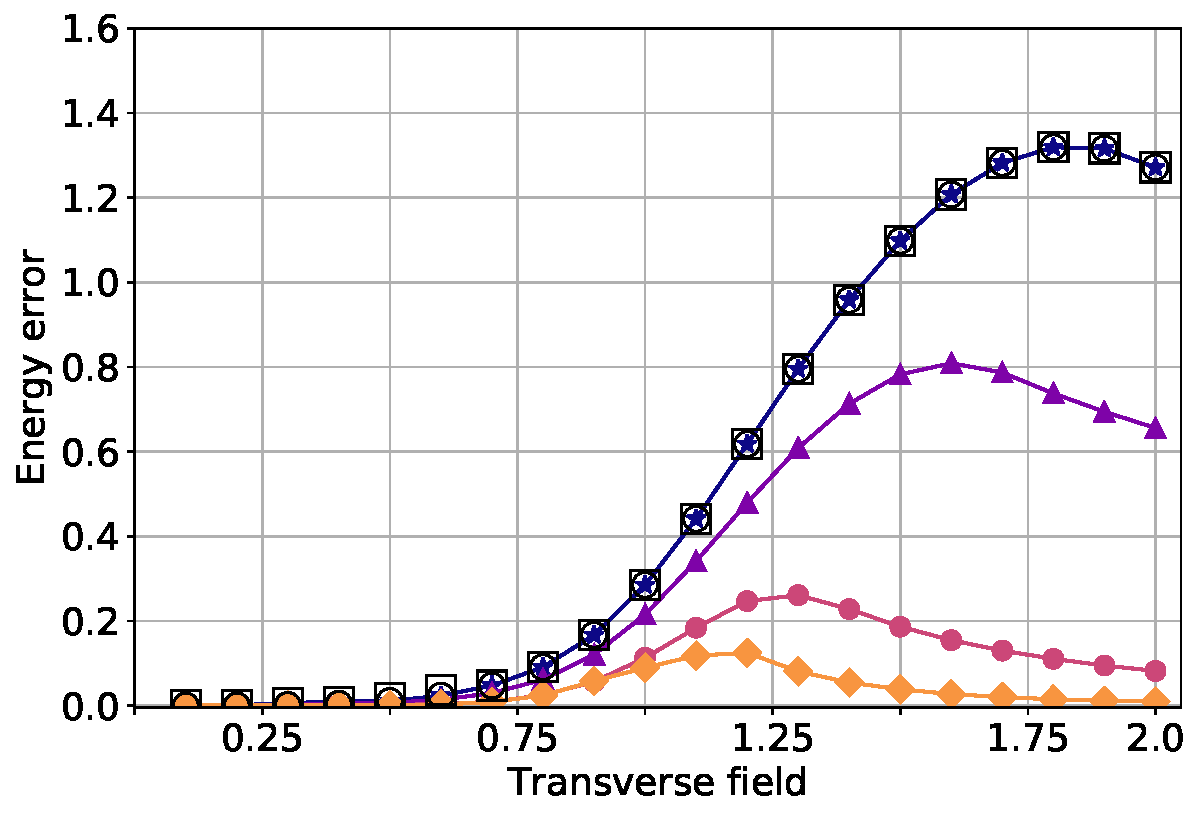
\includegraphics[width=0.7\textwidth]{../figures/dE_ising.pdf}
    \caption{Absolute value of the difference in energy between the exact solution and VQE solutions for the transverse field Ising model. Hollow squares: rank-1 ansatz, hollow circles: tree tensor network, filled markers: checkerboard states ($\bigstar$: 1 layer, $\blacktriangle$: 2 layers, $\bullet$: 3 layers, $\blacklozenge$: 4 layers). Reprinted from \cite{uvarov_machine_2020}.}
    \label{fig:dE_ising}
\end{figure}

The second model considered in this section is the Heisenberg XXZ model:

\begin{equation}
    \label{eq:heisenberg_xxz}
    H = \sum_{i=1}^n \left[J_\perp\left(X_i X_{i+1} + Y_i Y_{i+1}\right)
        + J_z Z_i Z_{i+1}\right].
\end{equation}

For this model, the error dependence was studied using the best ansatz among those studied for the TFI model. The solutions obtained using AAVQE were found to exhibit different behavior depending on the direction of movement through the parameter range (Fig.~\ref{fig:dE_xxz}).

\begin{figure}
    \centering
    \begin{subfigure}{.48\linewidth}
        \centering
        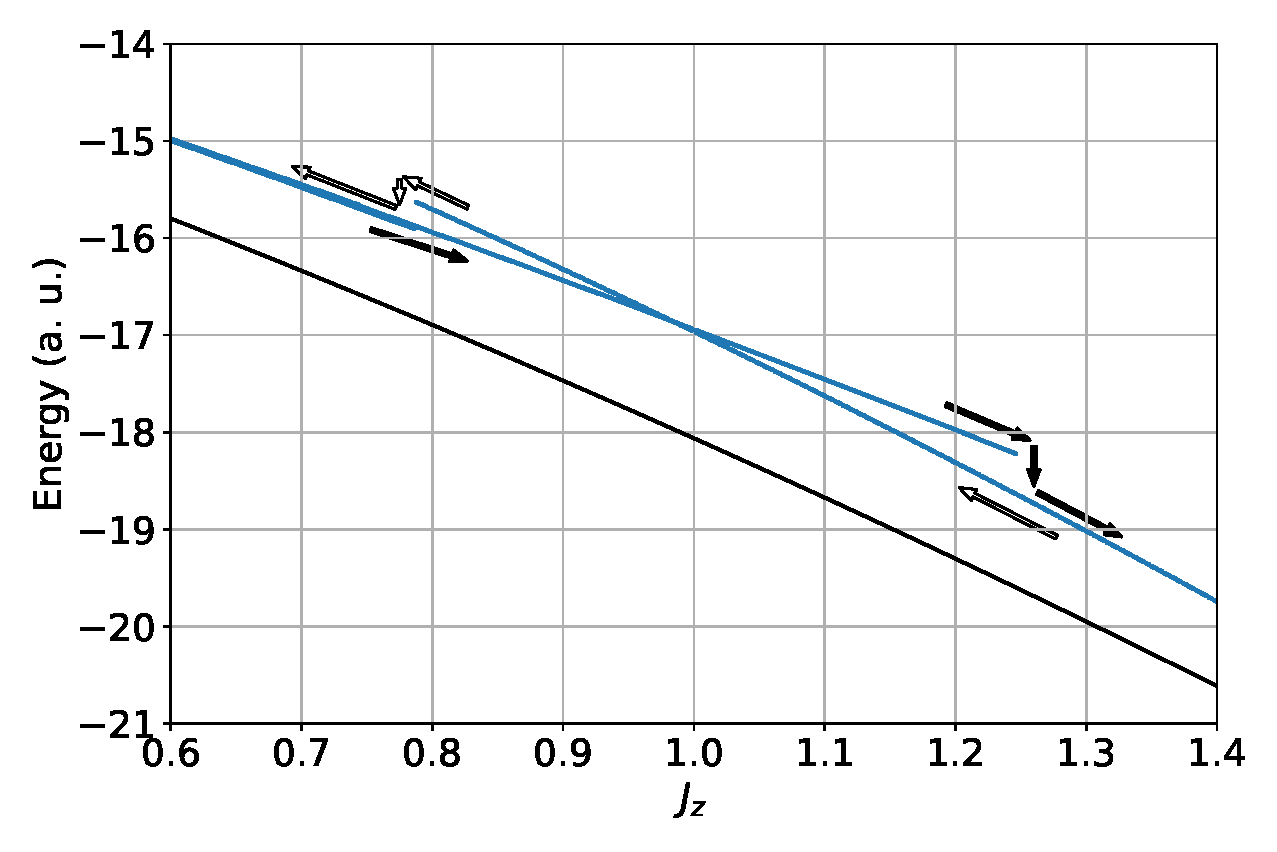
\includegraphics[width=\textwidth]{../figures/vqe_hysteresis_xxz_new.eps}
    \end{subfigure}\begin{subfigure}{.48\linewidth}
        \centering
        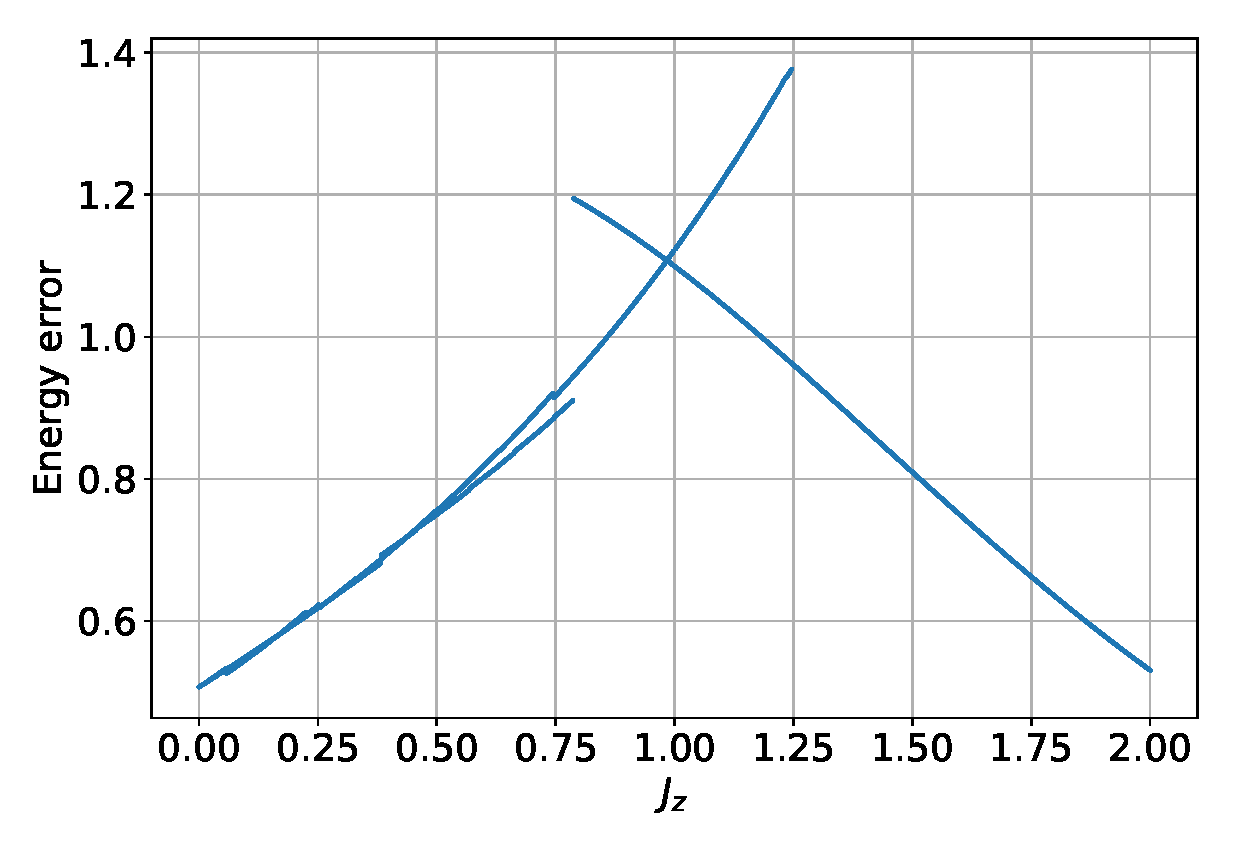
\includegraphics[width=\textwidth]{../figures/dE_xxz_best.eps}
    \end{subfigure}
    % 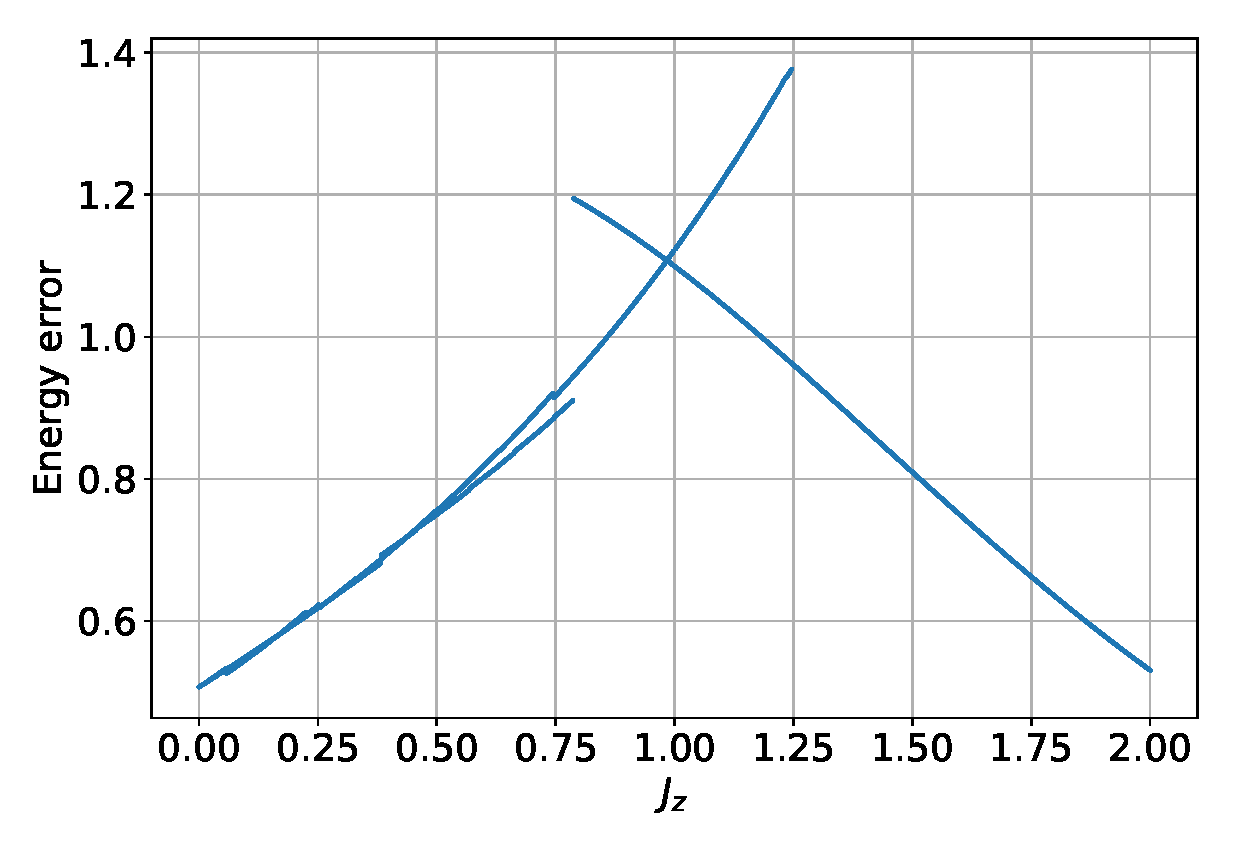
\includegraphics[width=0.7\textwidth]{../figures/dE_xxz_best.eps}
    \caption{Left: Ground-state energy estimate for the XXZ model found
    in VQE sweeps. Filled (empty) arrows guide the eye along the
    “up” (“down”) sweep. The black line denotes the energy of the exact solution. Reprinted from \cite{uvarov_machine_2020}. Right: Energy difference between the exact solution and the ansatz solutions for the XXZ model.}
    \label{fig:dE_xxz}
\end{figure}

Section 3.3 presents the results of simulating VQE for the Hubbard model. This model describes the behavior of fermions on a one-dimensional chain of sites, governed by Coulomb repulsion:

\begin{equation}
    H_{\text{Hubbard}} = \sum_{i \in [n], \sigma \in \{\uparrow, \downarrow\}} \epsilon_{i \sigma} \hat{n}_{i \sigma}
    - \sum_{<i, j>, \sigma \in \{\uparrow, \downarrow\}} t_{ij, \sigma} (a^\dagger_{i \sigma} a_{j \sigma} + a^\dagger_{j \sigma} a_{i \sigma})
    + U \sum_{i \in [n]} \hat{n}_{i \uparrow} \hat{n}_{i \downarrow},
\end{equation}

Our numerical experiments consider a simplified model, in which every site accommodates only one particle, and all particles are spinless. On the other hand, the Coulomb repulsion is extended to nearest-neighbor and next-nearest-neighbor sites:
\begin{equation}
    \label{eq:hubbard_nnn}
    H = - \sum_{<i, j>} t_{ij} (a^\dagger_{i} a_{j} + a^\dagger_{j} a_{i})
    + \sum_{i, j} U_{ij} \hat{n}_{i} \hat{n}_{j}.
\end{equation}
Here $t_{ij} = 1, U_{i, i+1} = V_1, U_{i, i+2} = V_2$, and all other terms $U_{ij}$ are zero.

The Hamiltonian was mapped to a spin Hamiltonian using the Jordan--Wigner transform. The numerical experiments use the checkerboard ansatz with two-qubit blocks preserving the number of particles \cite{barkoutsos_quantum_2018}:

\begin{equation}
\label{eq:particle-conserving_gate}
    U(\theta_1, \theta_2) = 
    \begin{pmatrix}
1 & 0 & 0 & 0 \\
0 & \cos{\theta_1} & e^{\imath \theta_2} \sin \theta_1 & 0 \\
0  & e^{-\imath \theta_2} \sin \theta_1  & -\cos{\theta_1} & 0  \\
0 & 0 & 0 & 1
\end{pmatrix}.
\end{equation}

Figure \ref{fig:vqe_hubbard_nnn} shows the results of VQE optimization for the model (\ref{eq:hubbard_nnn}) for different numbers of qubits and depths of the circuit. For the most part, the energy exhibits exponential convergence with the depth of the ansatz circuit, although the exact value of the exponent is different for different numbers of qubits. The jagged appearance of the curves is due to the fact that the specific particle-conserving gate used in the ansatz does not possess the identity gate in its configuration space. It is also clear that for larger $n$, the convergence tends to go slower. In particular, for $n=11$ qubits, the energy error remains roughly the same despite the increase in the number of layers.

\begin{figure}
    \centering
    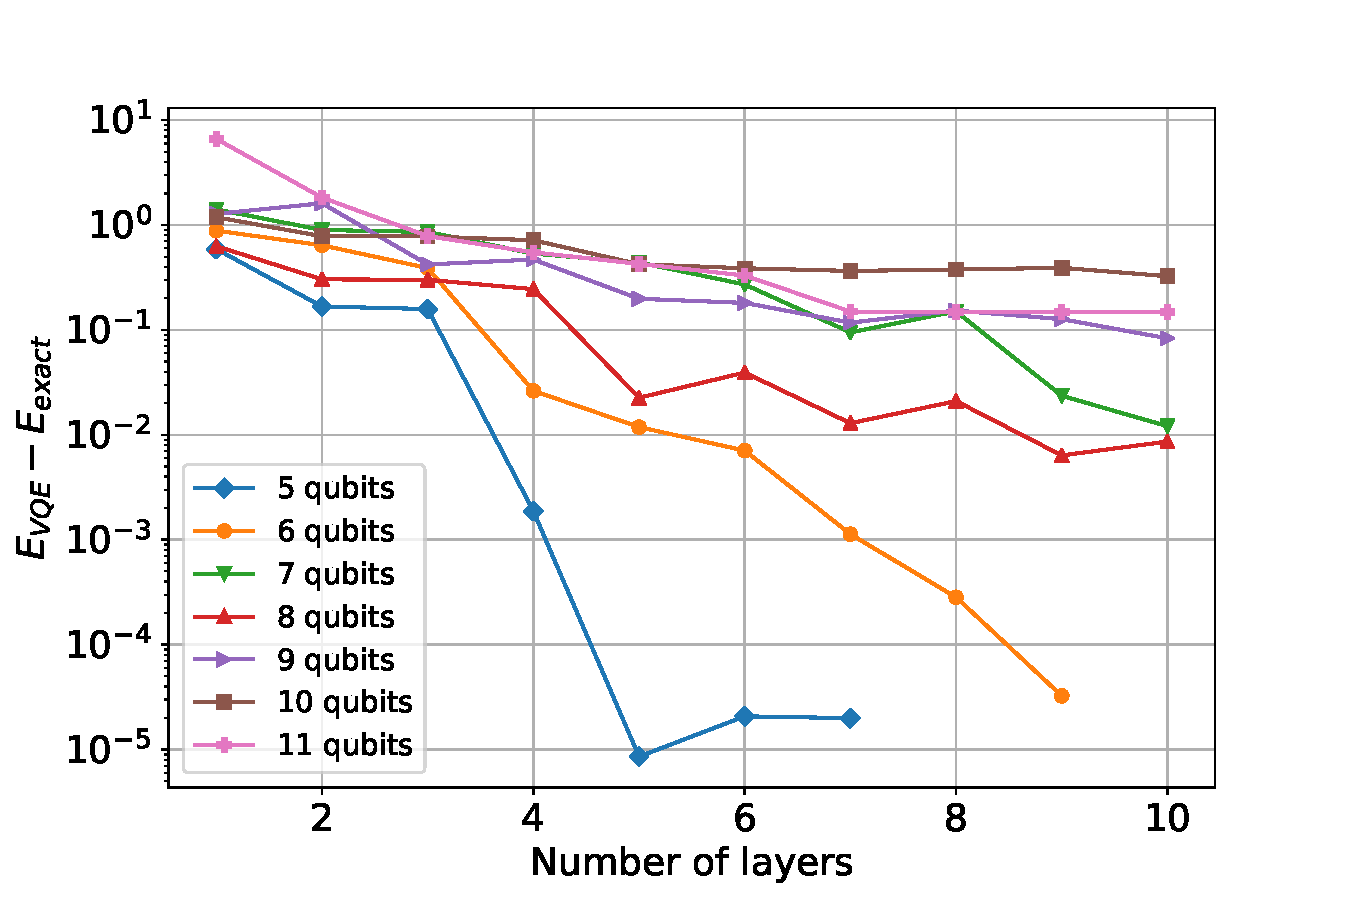
\includegraphics[width=0.7\textwidth]{../figures/vqe_hubbard_nnn.pdf}
    \caption{Convergence of the VQE solution to the true ground state for the 1D next-nearest-neighbor repulsion Hubbard model versus the number of layers, on condition $V_1 = 2t, V_2 = t$. Cases of $n \leq 4$ qubits are not shown as they converged to exact solution within 2 layers. Reprinted from \cite{uvarov_variational_2020}.}
    \label{fig:vqe_hubbard_nnn}
\end{figure}

In addition to the energy error of the numerical solutions, we studied the behavior of correlation functions. The results are shown in Fig.~\ref{fig:correlation}. While the qualitative agreement is evident, the accuracy of the approximation, as well as the size of the spin chain, were too low to produce any reasonable quantitative estimates of the asymptotical behavior of the correlation function.

\begin{figure}
    \centering
    \includegraphics*[width=0.7\textwidth]{../figures/Correlation.pdf}
    \caption{Density-density correlation function between spatially separated lattice sites. Filled dots denote exact values as obtained by virtue of exact diagonalization of the Hamiltonian (\ref{eq:hubbard_nnn}), dashed lines denote different approximations. Here $V_1 = 2t, V_2 = t$. Reprinted from \cite{uvarov_variational_2020}.}
    \label{fig:correlation}
\end{figure}

The final part of the section is devoted to studying the occurrence of the barren plateaus effect for the Hubbard model. The barren plateaus effect is an observation regarding the cost function landscape in variational quantum algorithms. For a sufficiently deep and expressive ansatz circuit, the derivative of the cost function becomes vanishingly small. Specifically, under the random choice of ansatz parameters, the expected value of all partial derivatives is zero, and the variance is exponentially small in the number of qubits $n$ \cite{mcclean_barren_2018}. This result, however, concerns very long circuits. The transient behavior of the derivatives is studied in this section.

Figure \ref{fig:plateaus_hubbard_ising}, top left, shows the behavior of the variance of the derivatives (averaged over random selections of $\boldsymbol{\theta}$ and $k$) for the next-nearest-neighbor Hubbard model (\ref{eq:hubbard_nnn}) under the Jordan--Wigner mapping. The particle-conserving ansatz is used for the analysis. For most qubit numbers and regardless of the model parameters, said variance drops to its limiting value even for very shallow circuits. In contrast, the same derivatives under the Bravyi--Kitaev mapping show a more gradual behavior (Figure \ref{fig:plateaus_hubbard_ising}, top right): the variance starts off by decaying exponentially with the depth, then saturates. The particle-preserving gate in the ansatz was replaced with a more generic gate, since the former would no longer conserve the particle number.
For comparison, we also performed a similar experiment for the transverse field Ising model. The gradient behavior away from the critical point ($h = 0.1$) and at the critical point ($h = 1$) is shown in Fig.~\ref{fig:plateaus_hubbard_ising}, bottom. In this case, the gradient variance decays exponentially with the number of layers until reaching the plateau regime for the particular number of qubits. Thus, for 4 qubits the plateau is reached right away, while for 10 qubits, 30 layers of the ansatz are still a number belonging to the transition regime. In the meantime, the criticality of the model does not seem to affect this behavior. A possible reason for the behavior observed in these three cases is that the Jordan--Wigner mapping produces highly nonlocal operators which are difficult to optimize.

\begin{figure}
    \centering
    \begin{subfigure}{.48\linewidth}
        \centering
        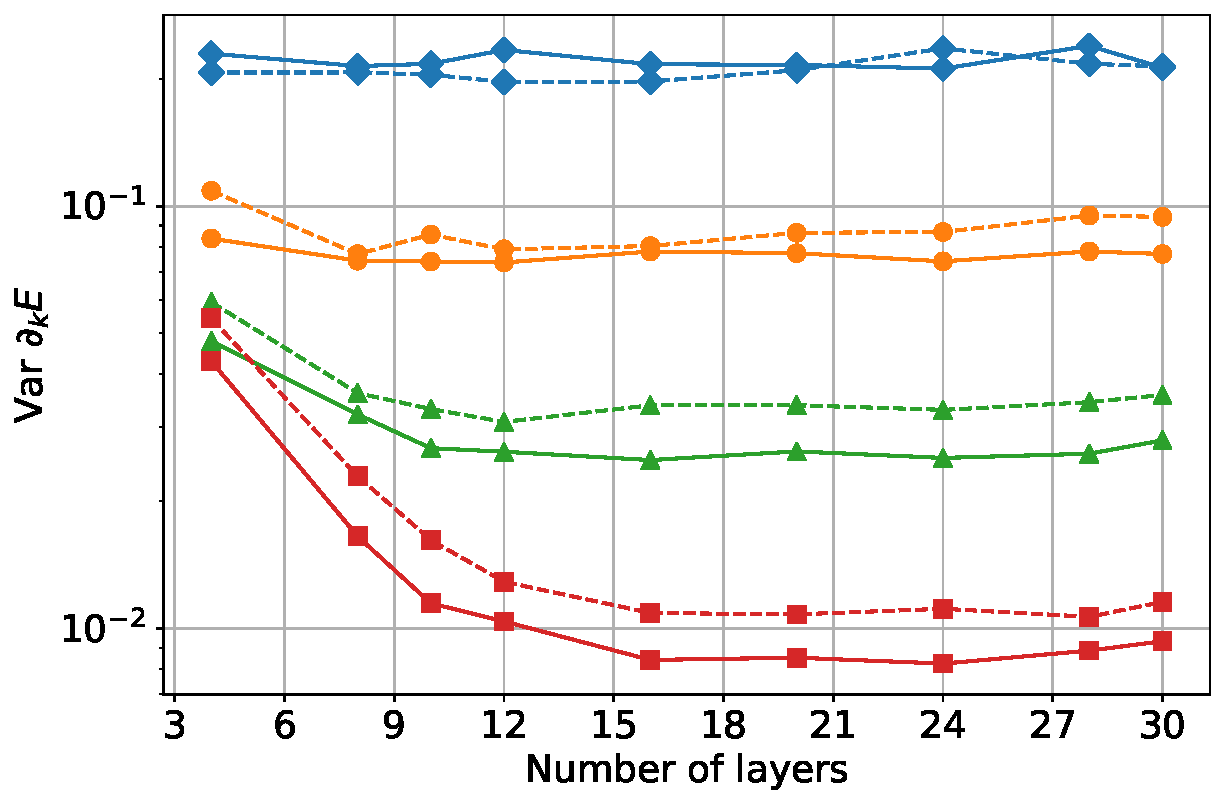
\includegraphics[width=\textwidth]{../figures/plateau_hubbard_jw_both.pdf}
    \end{subfigure}\begin{subfigure}{.48\linewidth}
        \centering
        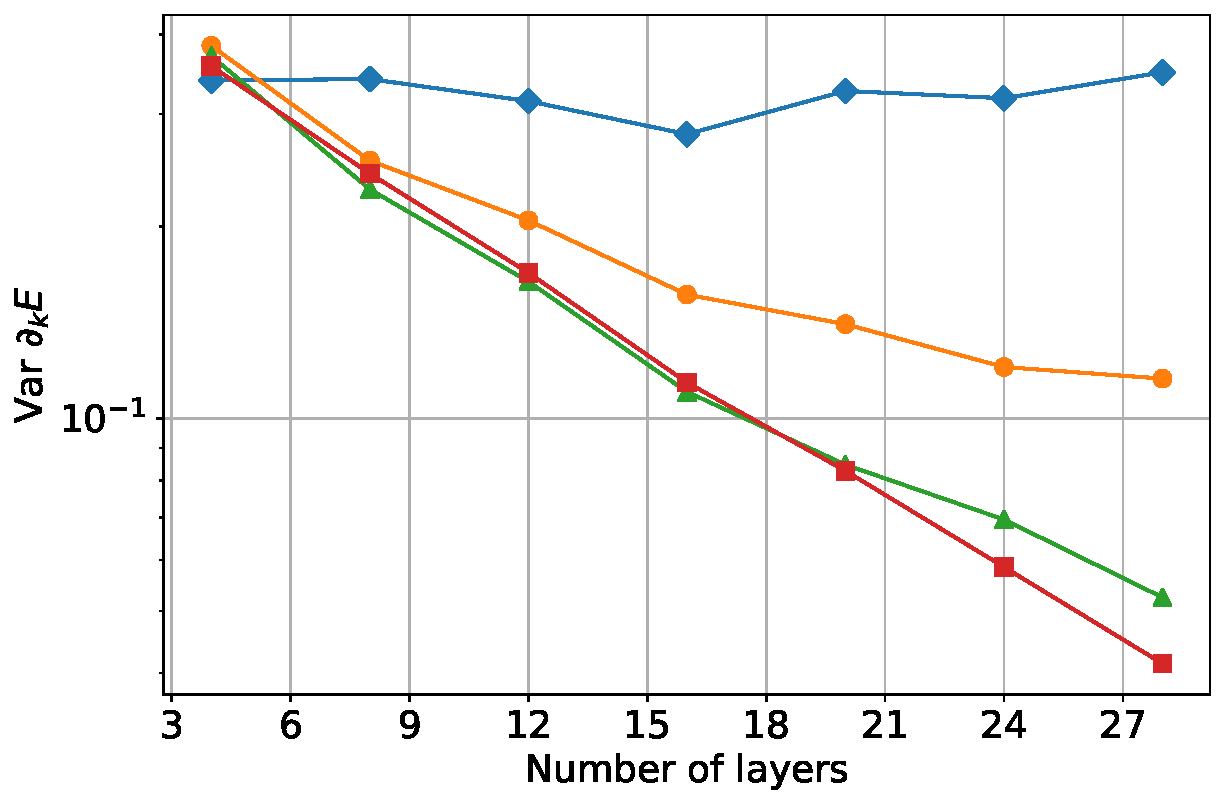
\includegraphics[width=\textwidth]{../figures/plateau_hubbard_bk.pdf}
    \end{subfigure}
    \begin{subfigure}{.48\linewidth}
        \centering
        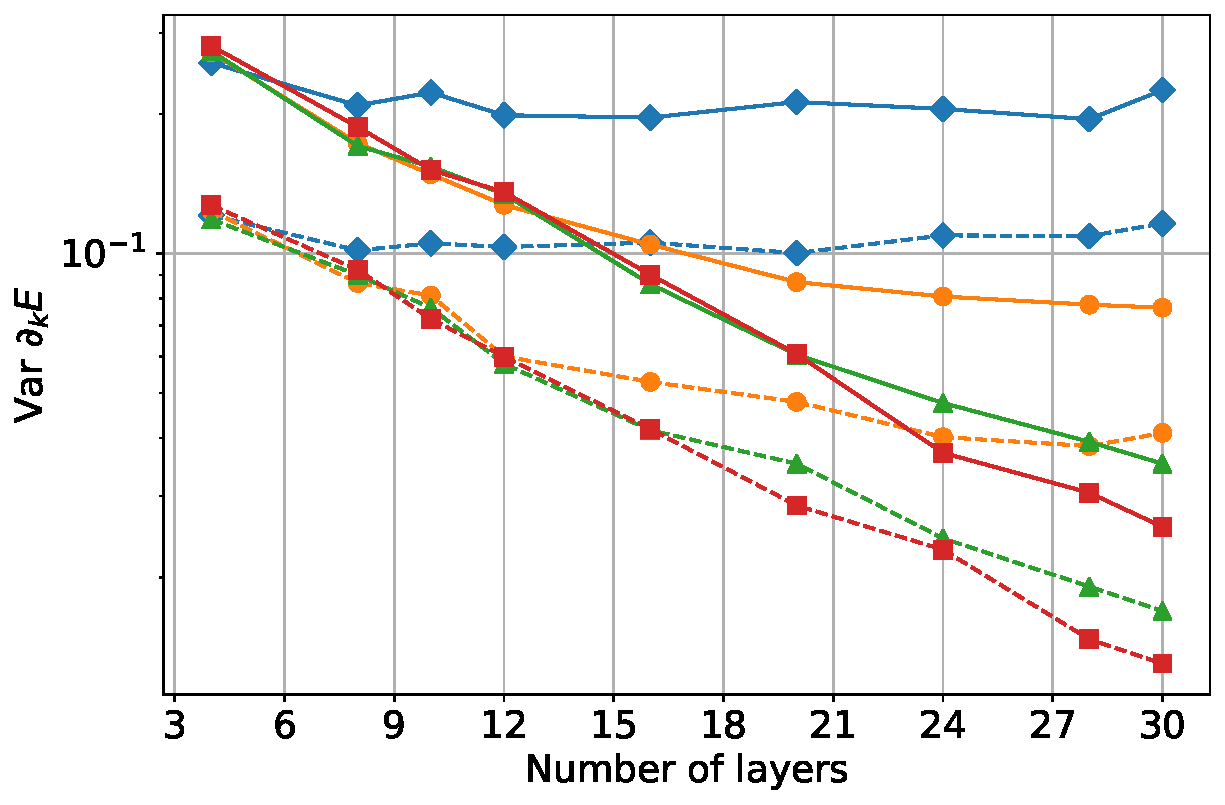
\includegraphics[width=\textwidth]{../figures/plateau_ising_both.pdf}
    \end{subfigure}
    \caption{\textbf{Top left:} barren plateau effect for the Hamiltonian of Eq. (3) with
    $V_1 = t$ and $V_2 = 0$ (dashed lines), as well as $V_1 = 2t$ and $V_2 = t$
    (solid lines) versus the number of qubits as realized by virtue of
    Jordan--Wigner mapping. Diamonds: four qubits; circles: six qubits;
    triangles: eight qubits; squares: 10 qubits. \textbf{Top right:} same effect under Bravyi--Kitaev mapping, $V_1 = 2t$, $V_2 = t$.
    \textbf{Bottom:} same effect for for the transverse field Ising model of Eq. (4) away from criticality with $h = 0.1$ (dashed lines) and at the critical point $h = 1$ (solid lines).    
    Reprinted from \cite{uvarov_variational_2020}.}
    \label{fig:plateaus_hubbard_ising}
\end{figure}

Section 3.4 contains concluding remarks. 

\textbf{The fourth chapter} discusses the possibility of applying VQAs to machine learning problems. Section 4.1 introduces the quantum approach to machine learning and reviews the existing literature on the topic. Section 4.2 presents our results in training a quantum classifier on quantum data obtained from VQE experiments. We start with the TFI model studied in the third chapter. This model has a phase transition point at $h=1$. Thus, the solutions obtained by VQE can be partitioned in two subsets: those for $h<1$ and those for $h>1$. The task of the classifier was to distinguish between these two classes. The data supplied to the classifier consisted of approximate ground states of Hamiltonians for different values of $h$.

\begin{figure}
    \centering
    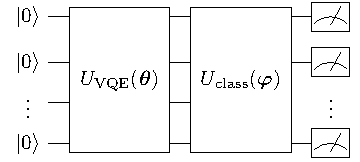
\includegraphics[width=0.7\linewidth]{../figures/classifier_circuit.pdf}
    \caption{Quantum circuit that implements the classifier. The first part prepares the VQE solution, the second one performs the classification. The assigned label is inferred from the measurements in the $Z$ basis. Both $U_{\mathrm{VQE}}$ and $U_{\mathrm{class}}$ have the checkerboard structure. Reprinted from \cite{uvarov_machine_2020}.}
    \label{fig:classifier_scheme}
\end{figure}

The classifier of quantum states is again a variational quantum circuit $U_{\mathrm{class}}$. The overall circuit is then the concatenation of the circuit preparing VQE solutions and the classifier circuit (Fig.~\ref{fig:classifier_scheme}). The label assigned by the neural network is proportional to the amount of qubits measured in the state ``1'', i.e.~the signal is the majority vote of the qubits. Effectively, estimating the majority is equivalent to estimating the energy of the state $U_{\mathrm{class}}(\boldsymbol{\varphi}) \ket{\psi(\boldsymbol{\theta})}$ relative to the following Hamiltonian:
\begin{equation}
    \label{eq:h_vote}
    H_{\text{vote}} = \sum_{w(i) > n/2} \ket{i} \bra{i} + \frac{1}{2}\sum_{w(i) = n/2} \ket{i} \bra{i}.
\end{equation}
Here $w(i)$ denotes the Hamming weight of the basis state $\ket{i}$, i.e.~the number of ones it contains.

To train the classifier circuit $U_{\mathrm{class}}(\boldsymbol{\varphi})$, we used the log-likelihood cost function. Let $\{ (\boldsymbol{\theta}_i, y_i) \}_{i=1}^{N_{train}}$ be the set of training data points and their labels, $y_i \in \{0, 1\}$. Let $p_i \in [0, 1]$ be the label predicted by the neural network:
\begin{equation}
    p_i = \bra{\psi(\boldsymbol{\theta}_i)} U^\dagger_{\mathrm{class}} (\boldsymbol{\varphi})H_{\text{vote}} U_{\mathrm{class}}(\boldsymbol{\varphi})\ket{\psi(\boldsymbol{\theta}_i)}.
\end{equation}
Then the loss function is:
\begin{equation}
\label{eq:logloss}
    f = -\sum_{i=1}^{N_{train}} \left( y_i \log p_i + (1 - y_i) \log (1 - p_i) \right).
\end{equation}
The classifier was successfully trained to distinguish the phases in the TFI model with 97\% accuracy (Fig.~\ref{fig:phase_classification}, left).

The next part of the section reports the same experiment for the Heisenberg XXZ model (\ref{eq:heisenberg_xxz}). This model also has a phase transition point at $J_z = 1$, $J_\perp = 1$, however in this case, it is more complicated to detect. As a result, the classifier circuit has to be extended by 2 layers. Another complication comes from the rotational symmetry of the model. Nonetheless, the classification was still performed successfully, albeit at a lower accuracy of 93\% (Fig.~\ref{fig:phase_classification}, right). 

The final paragraph of the section presents the test of the classifier on a model constructed by using two random Hamiltonians: $H(\alpha) = (1 - \alpha) H_1 + \alpha H_2, \ \alpha \in [0, 1]$, where $H_1$ and $H_2$ are random Hermitian matrices sampled from the Gaussian unitary ensemble. We split solutions in two classes: (i) $\alpha < 0.5$ and (ii) $\alpha > 0.5$. Then we run the optimization routine to train the learning circuit to discern between the two  classes. The accuracy in this experiment reached 93\%.


\begin{figure}
    \centering
    \begin{subfigure}{.48\linewidth}
        \centering
        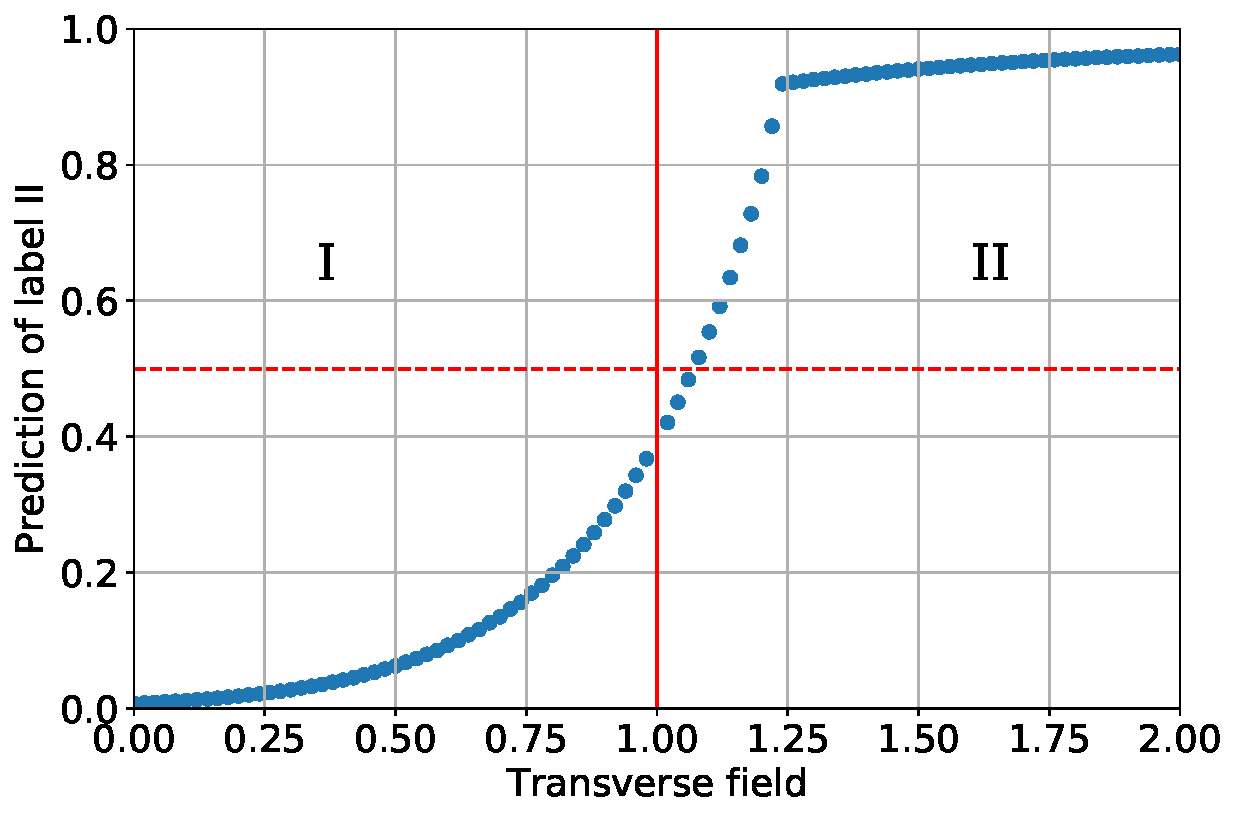
\includegraphics[width=\textwidth]{../figures/tfi_classification_new_2021}
    \end{subfigure}\begin{subfigure}{.48\linewidth}
        \centering
        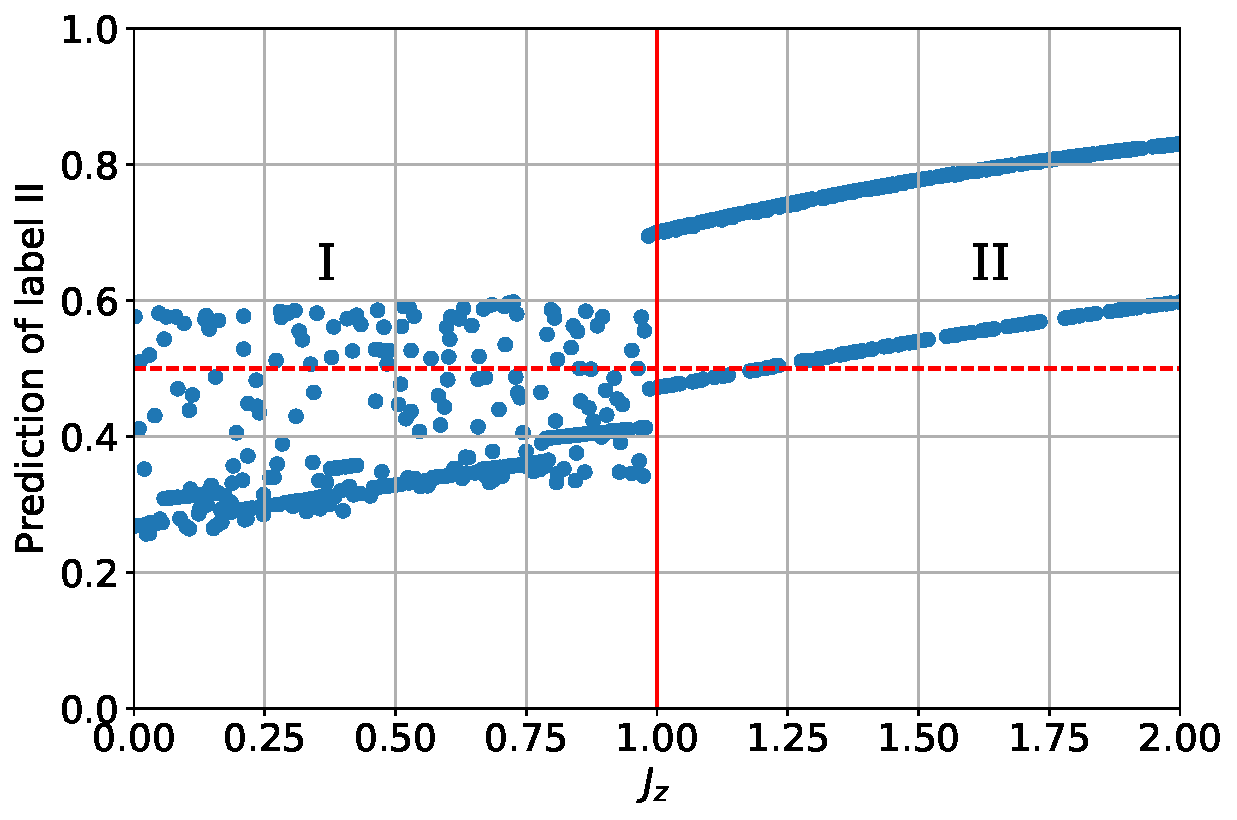
\includegraphics[width=\textwidth]{../figures/xxz_classification_new_2021.pdf}
    \end{subfigure}
    \caption{Left: predicted label of phase II as a function of magnetic field for transverse field Ising model. Right: predicted label of phase II as a function of $J_z$ for the XXZ model. Roman numbers denote the phases I and II of the models.}
    \label{fig:phase_classification}
\end{figure}

Section 4.3 discusses the possible alternative setups in quantum classification. One modification of the protocol is called learning by confusion: when we don't know the location of the phase transition point, we partition the examples with respect to a guess point $h^*$, then compare the results for different values of $h^*$ and pick the one with the best test accuracy \cite{van_nieuwenburg_learning_2017}. We present a simple test of that approach and observe that it successfully predicts the phase transition point. Another important choice in the setup is the cost function. We discuss measuring just the first qubit as a possible alternative. The conclusions of the chapter are given in Section 4.4.

\textbf{The fifth chapter} presents the results of our study of the barren plateaus phenomenon, previously encountered in the third chapter. Section 5.1 introduces the Haar measure and integration with respect to it. 
\begin{definition}
    The \textit{Haar measure} $\mu: \mathrm{Borel} (U(d)) \rightarrow [0, 1]$ on the unitary group $U(d)$ is the unique left- and right-invariant probability measure on that group. That is, let $V \in U(d)$ and let $\mathcal{A} \in \mathrm{Borel} (U(d))$. Then $\mu(\mathcal{A}) = \mu(V \mathcal{A}) = \mu(\mathcal{A} V)$.
\end{definition}
The main results presented in this section are two integrals over the Haar measure:
\begin{equation}
    \label{eq:haar_integral_1}
    \int U^\dagger A U \mathrm{d} \mu = \frac{\operatorname{Tr} A}{d} \cdot I
\end{equation}
\begin{align}
    \label{eq:haar_integral_2}
     \int (U^\dagger \otimes U^\dagger) (A \otimes B) (U \otimes U) \mathrm{d} \mu & = 
      \frac{1}{d^2 - 1} \left[  
         (\Tr A \Tr B  - \frac{1}{d} \Tr AB) \mathbbm{1} \otimes  \mathbbm{1} + \right. \\
       &  \left. + (\Tr AB  - \frac{1}{d} \Tr A \Tr B) \mc{S} \right].
\end{align}
Here $A, B \in \operatorname{End}(\mathbb{C}^d)$ are arbitrary linear operators, and $\mc{S}$ denotes a swap of two tensor components: $\mc{S} (v \otimes w) = w \otimes v$.

Section 5.2 introduces the $t$-designs, which are unitary ensembles that mimic the lowest moments of the Haar distribution while possibly being easier to sample from.
\begin{definition}
    A probability distribution $\nu$ on the unitary group $U(2^n)$ is a  \textit{unitary} $t$\textit{-design}
    if the expected value of any polynomial of power $t$ in the matrix elements of $U$ and $U^*$ with respect to $\nu$ is the same as that w.r.t.~the Haar measure on $U(2^n)$.  
\end{definition}
We also introduce so-called \textit{approximate $t$-designs} and \textit{tensor product expanders}. There are many definitions for different purposes \cite{low_pseudo-randomness_2010}, but we picked those that we found the most convenient for a numerical experiment.
\begin{definition}
    An ensemble of random unitary gates $\nu$ is a $\lambda$-approximate tensor product expander (TPE) if $||\mathbb{E}_{Haar} (U^{\otimes t} \otimes (U^*)^{\otimes t}) - \mathbb{E}_\nu (U^{\otimes t} \otimes (U^*)^{\otimes t}) ||_p \leq \lambda$ for $p=\infty$. When such an equation holds for $p=1$, the ensemble $\nu$ is called a $\lambda$-approximate $t$-design.
\end{definition}
Section 5.3 formally introduces the barren plateaus phenomenon. We consider a parametrized quantum circuit in which we distinguish one gate: $U = U_A e^{-\mathrm{i} \theta F} U_B$, where $F$ is a Pauli string. Let our cost function be some local Hamiltonian $H = \sum c_i h_i$, where $h_i$ are Pauli strings, and $h_0 = I$. The energy to be minimized in VQE is then equal to 

\begin{equation}
    E = \bra{\psi_0} U_B^\dagger e^{\mathrm{i} \theta F} U_A^\dagger H U_A e^{-\mathrm{i} \theta F} U_B \ket{\psi_0}.    
\end{equation}

The energy derivative over $\theta$ is now equal to 

\begin{multline}
    \label{eq:partial_E}
    \partial_\theta E = \bra{\psi_0} U_B^\dagger e^{\mathrm{i} \theta F} (\mathrm{i} F) U_A^\dagger H U_A e^{-\mathrm{i} \theta F} U_B \ket{\psi_0} + \\
    +
    \bra{\psi_0} U_B^\dagger e^{\mathrm{i} \theta F} U_A^\dagger H U_A (-\mathrm{i} F) e^{-\mathrm{i} \theta F} U_B \ket{\psi_0} = \\
    = \mathrm{i} \bra{\psi_0} U_B^\dagger e^{\mathrm{i} \theta F}  [F, U_A^\dagger H U_A] e^{-\mathrm{i} \theta F} U_B \ket{\psi_0}.
\end{multline}

In this setup, the phrase ``barren plateaus'' refers to the following theorem, which is proven in the remainder of the section:

\begin{theorem}[after \cite{mcclean_barren_2018}]
    \label{thm:mcclean}
    Let either $U_A$ or $U_B$ form a $2$-design. If $\operatorname{card} H \in \operatorname{poly}(n)$, and the Pauli coefficients $c_i$ are bounded by a constant, then the variance $\operatorname{Var} \partial_\theta E \in O(2^{-n})$.
\end{theorem}

Section 5.4 reports on our theoretical contribution to the study of barren plateaus. We introduce the following definitions.

\begin{definition}[Super Pauli strings]
    If $h$ is a Pauli string, then we will call $h \otimes h$ the induced \emph{super Pauli string}. If a Pauli string acts on qubits labeled $1, 2, \dots, n$, then a super Pauli string acts on qubits labeled $1, 2, \dots, n, 1', 2', \dots, n'$.
\end{definition}

\begin{definition}[Causal cone] 
    Let $U$  be an ansatz, and $h$ a Pauli string. 
    A gate (or a block of gates) $V$ is in the \emph{causal cone} $C(h, U)$ of $h$ under ansatz $U$, if that gate or block cannot be eliminated from the conjugate $U^\dagger h U$. We denote as $|C(h, U)|$ the support of this causal cone, i.e.~the number of qubits on which $U^\dagger h U$ can act nontrivially.
\end{definition}


\begin{definition}[Mixer]

    Let $\mc{Y}$ be a subset of the qubit registry. Define the \textit{local mixing operator}, or simply a \textit{mixer}\footnote{The mixer is in fact a quantum channel since it is defined by its own Kraus decomposition.}  $M_{\mc{Y}}: \operatorname{End} (\mc{H}\otimes \mc{H}) \rightarrow \operatorname{End} (\mc{H}\otimes \mc{H})$ as follows:
    \begin{equation}
    \begin{aligned}
        \label{eq:m2}
        & M_{ \mc{Y}} (h_1 \otimes h_2) = \int d\mu_{\mc{Y}} (U)
        (U^\dagger \otimes U^\dagger)
        (h_1 \otimes h_2)
        (U \otimes U),
    \end{aligned}{}
    \end{equation}{}
    where $\mu_{\mc{Y}}$ is the Haar distribution of unitary operators acting nontrivially on $\mc{Y}$ and trivially on all other qubits.
    
\end{definition}

The mixer can act on super Pauli strings by conjugation. The results of this action are formulated in the following propositions.

\begin{proposition}
    \label{prop:m2_decomposed}
    Let $h$ be a Pauli string. If its substring $h_{\mc{Y}}$ is nontrivial, then
    
    \begin{equation}
        M_{\mc{Y}}(h \otimes h) = \frac{1}{4^{|\mc{Y}|} - 1} \left( \sum_{\sigma_\mc{Y} \neq \mathbbm{1}} (\sigma_{\mc{Y}} \otimes h_{\mc{H} \setminus \mc{Y}})^{\otimes 2}\right),
    \end{equation}{}
    where the summation extends over all nontrivial Pauli substrings $\sigma_{\mc{Y}}$.
    Otherwise,  $M_{\mc{Y}}(h \otimes h) = h \otimes h$.
    
\end{proposition}

\begin{proposition}
    \label{prop:mixer_kills_asymmetry}
    Let $h_1, h_2$ be Pauli strings such that their restriction on a registry $\mc{Y}$ is different. Then $\mc{M_Y} (h_1 \otimes h_2) = 0$.
\end{proposition}

\begin{proposition}
    \label{prop:paulis_decouple}
    Let $\mc{Y}_1, ..., \mc{Y}_N$ be a collection of qubit subsets
    such that $\mc{Y}_1 \cup ... \cup \mc{Y}_N$ contains all $n$ qubits (the subsets are allowed to intersect). Let $h_1, h_2$ be two distinct Pauli strings. Then, 
    $M_{ \mc{Y}_N} \circ \dots \circ  M_{ \mc{Y}_1} (h_1 \otimes h_2) = 0.$
\end{proposition}

Next, we introduce a commutator operator $\mc{C}_{F} \in \operatorname{End}(\mc{H} \otimes \mc{H})  \rightarrow \operatorname{End}(\mc{H} \otimes \mc{H})$, which maps $A \otimes B$ to $[\rmi F, A] \otimes [\rmi F, B]$. Unlike the mixer operator, $\mc{C}_F$ is no longer a quantum channel since it does not preserve trace. Graphically, we can express this superoperator like this:

\newcommand{\legw}{1}
\newcommand{\gapw}{2}
\newcommand{\gaph}{1}
\newcommand{\barh}{0.6}
\newcommand{\wireh}{0.2}
\newcommand{\wiregap}{0.5}
\newcommand{\wirel}{0.3}

\begin{equation}
    \mc{C}_F(\star) =
    \adjustbox{raise=-7pt}{
    \begin{tikzpicture}[thick,scale=0.5]
    \node[blank] at (\gapw/2 + \legw, \gaph/2) {$\star$};
    
    
    \draw 
    (0, 0) 
    -- (0, \gaph + \barh) 
    -- (\gapw + \legw + \legw,\gaph + \barh)
    -- (\gapw + \legw + \legw,0)
    -- (\gapw + \legw,0)
    -- (\gapw + \legw, \gaph)
    -- (\legw, \gaph)
    -- (\legw,0)
    -- (0, 0)
    
    (0, \wireh) -- (-\wirel, \wireh)
    (0, \wireh + \wiregap) -- (-\wirel, \wireh + \wiregap)
    
    (\legw, \wireh) -- (\legw + \wirel, \wireh)
    (\legw, \wireh + \wiregap) -- (\legw + \wirel, \wireh + \wiregap)
    
    (\legw + \gapw, \wireh) -- (\legw + \gapw - \wirel, \wireh)
    (\legw + \gapw, \wireh + \wiregap) -- (\legw + \gapw - \wirel, \wireh + \wiregap)
    
    (\gapw + \legw + \legw, \wireh) -- (\gapw + \legw + \legw + \wirel, \wireh)
    (\gapw + \legw + \legw, \wireh + \wiregap) -- (\gapw + \legw + \legw + \wirel, \wireh + \wiregap)
    
    ;
    \end{tikzpicture}
    }
\end{equation}

\begin{proposition}
    \label{prop:commutator_old}
    The following identities hold:
    \begin{enumerate}
        \item For every $F \in \mathrm{Herm}(\mc{Y})$, $\mc{C}_{F}(\id_{\mc{Y}} \otimes \id_{\mc{Y}})$ vanishes. Thus, $M_{\mc{Y}} \circ \mc{C}_F \circ M_{\mc{Y}} (\id_{\mc{Y}} \otimes \id_{\mc{Y}})=0$.
        \item Let $F$ be a nontrivial Pauli string acting on $\mc{Y}$. Then, for any nontrivial Pauli string $h$ acting on $\mc{Y}$
        \begin{equation}
            \label{eq:sandwiched_commutator}
             M_{\mc{Y}} \circ \mc{C}_{F} \circ M_{\mc{Y}} \left( h^{\otimes 2}\right) = \frac{2 \cdot 4^{|\mc{Y}|}}{4^{|\mc{Y}|} - 1} M\left( h^{\otimes 2}\right).
        \end{equation}
    \end{enumerate}{}
\end{proposition}{}

In subsection 5.4.2 we are ready to formulate the main statements of the chapter.

\begin{theorem}
    \label{thm:block_plateaus}
    Let $H$ be an $n$-qubit Hamiltonian consisting of Pauli strings $h_i$: $H = \sum c_i h_i$ with finite $c_i \in \mathbb{R}$. Let the ansatz $U$ consist of $l$ layers, and denote $l_c$ the layer which contains the block $G_k$ depending on parameter $\theta_a$. 
    % \textcolor{blue}{\textbf{[I don't think we should write $\theta_k$; a block typically depends on more than one parameter. Maybe we can highlight its special role in some other way, like $\tilde{\theta}$ or $\hat{\theta}$? --- Alexey]}}. 
    Let each block of the ansatz be an independently parametrized local 2-design. Let the block $G$ also be decomposable into $G = G_A e^{-i \theta_a F} G_B$, where $G_A$ and $G_B$ are local 2-designs not depending on $\theta_a$. Then, the variance of the gradient of $E$ with respect to that parameter is bounded below as follows:
    
    \begin{equation}
        \operatorname{Var} \partial_a E \geq \frac{2 \cdot 4^{|\mc{Y}_k|}}{4^{|\mc{Y}_k|} - 1} \left( \frac34 \right)^{l - l_c}  \sum_i c_i^2 \cdot 3^{-|C(h_i, U)|},
    \end{equation}{}
    where $|C(h_j, U)|$ is the number of qubits in the causal cone of the $j^{th}$ Pauli string, and the summation is over those Pauli strings whose causal cone contains the block $G$.
\end{theorem}{}

The proof of this theorem uses the fact that $\partial_a E (h_i)$ are uncorrelated random variables:

\begin{proposition}
\label{lemma:expectations_decouple}
In the conditions of Theorem \ref{thm:block_plateaus}, the individual Pauli string coefficients make independent contributions to the total variance:
\begin{equation}
    \operatorname{Var} \partial_a E (H) = \sum_i c_i^2 \operatorname{Var} \partial_a E (h_i).
\end{equation}
\end{proposition}

The rest of the section first offers a brief idea of the proof, then goes through the proof in detail.

\begin{figure}
    \centering
    \begin{subfigure}{.48\linewidth}
        \centering
        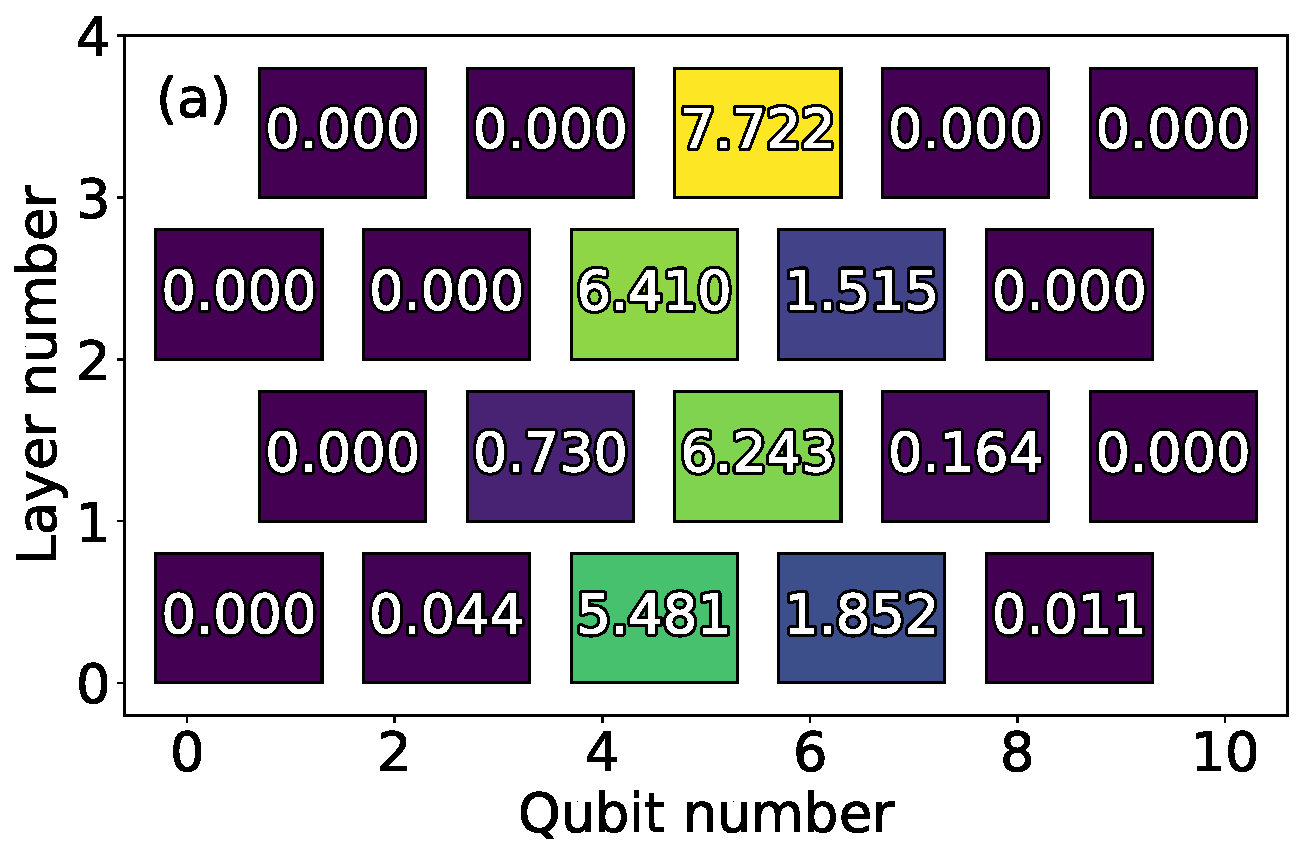
\includegraphics[width=\textwidth]{../figures/X5_ising.pdf}
    \end{subfigure}\begin{subfigure}{.48\linewidth}
        \centering
        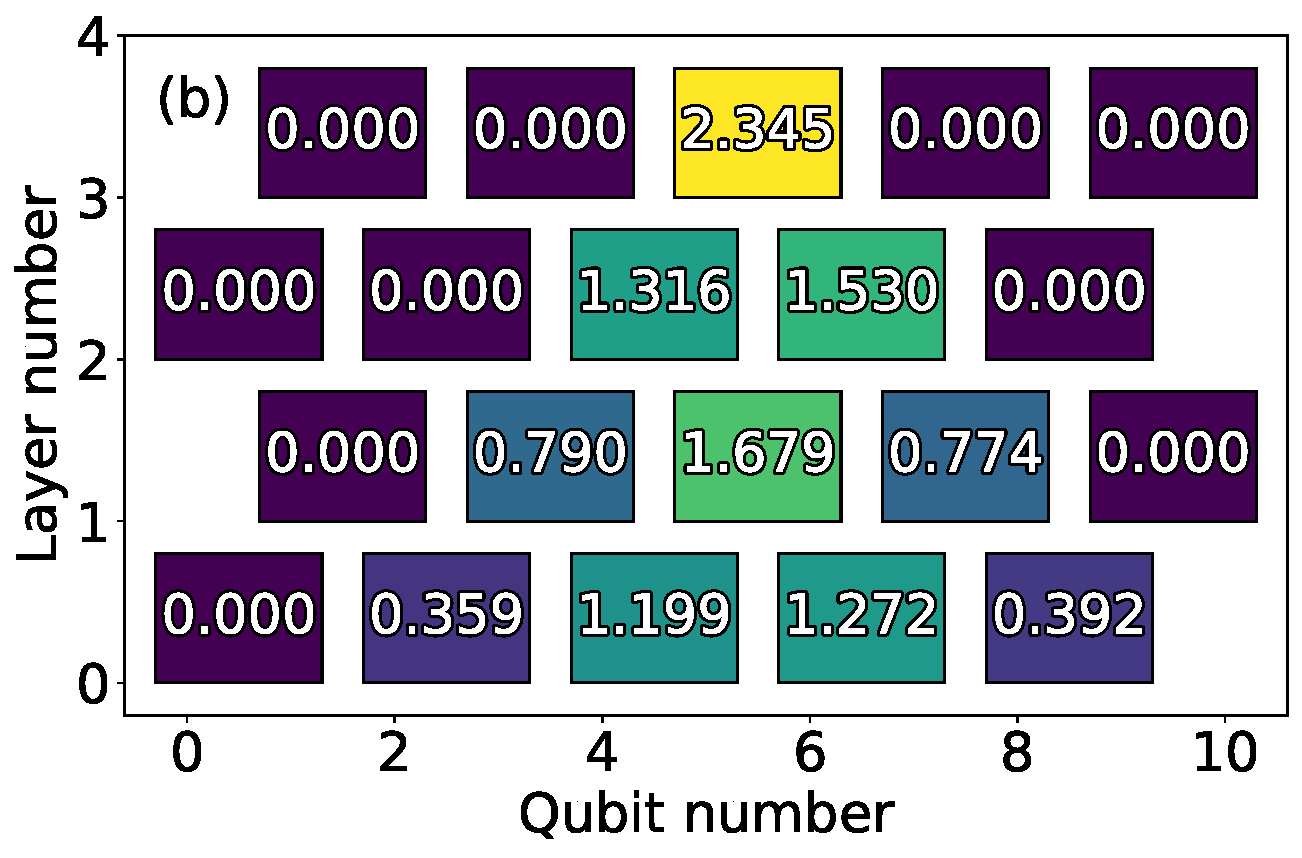
\includegraphics[width=\textwidth]{../figures/X5_cartan.pdf}
    \end{subfigure}
    \begin{subfigure}{.48\linewidth}
        \centering
        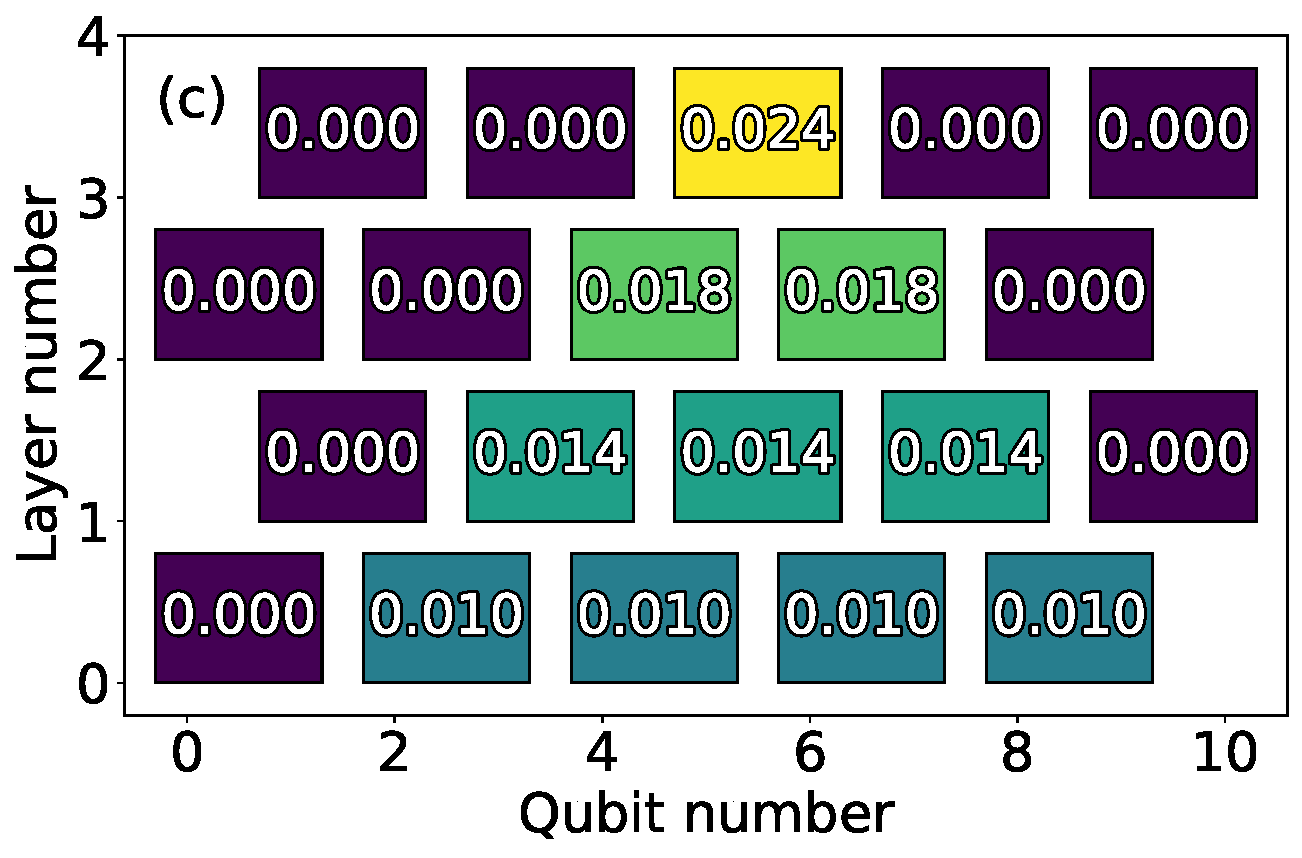
\includegraphics[width=\textwidth]{../figures/X5_theory.pdf}
    \end{subfigure}
    \caption{Derivative variances for $H = X_5$, averaged over parameters in each ansatz block. The numbers in the boxes denote $\Var \partial_\theta E \cdot 100$. Qubit number 10 is identified with qubit number 0. (a) Numerical result for an ansatz with blocks of $X,Z,ZZ$ rotations. (b) Numerical result for blocks implemented according to the Cartan decomposition. (c) Lower bound given in Theorem \ref{thm:block_plateaus}. Reprinted from \cite{uvarov_barren_2021}.}
    \label{fig:one-local}
\end{figure}

Section 5.5 presents numerical experiments supporting the main claims of the paper. The bound proven in Theorem \ref{thm:block_plateaus} holds in all cases considered, however it appears to be quite loose (e.g.~Fig.~\ref{fig:one-local}). The behavior of the derivatives also depends strongly on the choice of the blocks comprising the ansatz.
To justify the assumption that local circuit blocks are approximate 2-designs, we estimated their proximity by different norms. The results are shown in Table \ref{thm:block_plateaus}. 

\begin{table}
    \centering
    \begin{tabular}{|c|c|c|c|}
    \hline
        Block & 
        % Circuit diagram or matrix & 
        $\lambda_1$ & $\lambda_\infty$ & $\lambda_2$\\
        \hline
        $X$, $Z$, and $ZZ$ rotations &  
            % $\Qcircuit @C=1.0em @R=1.0em {
            %        \quad & \gate{R_Z} & \multigate{1}{R_{ZZ}} & \gate{R_X} & \qw \\
            %        \quad & \gate{R_Z} & \ghost{R_{ZZ}} & \gate{R_X} & \qw \\
            %    }$ &
        0.95 & 1.80 & 0.87\\
        \hline 
        Universal gates and a CNOT &
        %     $\Qcircuit @C=1.0em @R=1.0em {
        %    \quad & \gate{U_3} & \ctrl{1} & \gate{U_3} & \qw \\
        %    \quad & \gate{U_3} & \targ & \gate{U_3} & \qw \\
        %     }$
        % & 
        0.68 & 0.69 & 0.42\\
        \hline
        $Y$ rotations and a CZ \cite{cerezo_cost-function-dependent_2020} &            
        %     $\Qcircuit @C=1.0em @R=1.0em {
        %    \quad & \gate{R_Y} & \ctrl{1} & \gate{R_Y} & \qw \\
        %    \quad & \gate{R_Y} & \ctrl{-1} & \gate{R_Y} & \qw \\
        %     }$ 
            % & 
            1.76 & 1.76 & 1.00\\
        \hline
        Number-conserving \cite{barkoutsos_quantum_2018} & 
        % $
        % \begin{pmatrix}
        % 1 & 0 & 0 & 0 \\
        % 0 & \cos(\theta_1) & e^{i\theta_2} \sin(\theta_1) & 0 \\
        % 0 & e^{-i\theta_2} \sin(\theta_1) & -\cos(\theta_1) & 0 \\
        % 0 & 0 & 0 & 1 \\
        % \end{pmatrix}
        % $
        % & 
        2.40 & 2.40 & 1.00\\
        \hline
        Cartan decomposition \cite{khaneja_cartan_2000,khaneja_time_2001} &
    %     $\Qcircuit @C=1.0em @R=1.0em {
    %    \quad & \gate{U_3} & \multigate{1}{R_{XX}} & \multigate{1}{R_{YY}} & \multigate{1}{R_{ZZ}}& \gate{U_3} & \qw \\
    %    \quad & \gate{U_3} & \ghost{R_{XX}} & \ghost{R_{YY}} & \ghost{R_{ZZ}} & \gate{U_3} & \qw \\
    %     }$
    %         & 
            0.25 & 0.25 & 0.17\\
    \hline
    \end{tabular}
    \caption{Proximity to the 2-tensor product expander for different two-qubit blocks, estimated by random sampling. Circuit diagrams of ansatz blocks are given in the text of the dissertation.}
    \label{tab:local_designs}
\end{table}

Section 5.6 contains concluding remarks.

\textbf{The sixth chapter} proposes and analyzes a protocol for estimating the fidelity of Clifford states. Specifically, the chapter is focused on the Greenberger-Horne-Zeilinger (GHZ). This state is a popular target state for demonstration of all-to-all entanglement of qubits.
Section 6.1 reviews the techniques used in the literature to measure the fiedlity of the GHZ state: these methods involve measuring parity oscillations (PO) and multiple quantum coherences (MQC). 
Section 6.2 presents the mathematical tools required for the proposed method.

\begin{proposition}[Stability lemma]
    \label{prop:stability}
    Let $H$ be a Hamiltonian with eigenvalues $0 = \lambda_0 < \Delta = \lambda_1 \leq \lambda_2 \leq ... \leq \lambda_{\mathrm{max}}$ and corresponding eigenvectors $\ket{\lambda_i}$. Let $\rho$ be a density operator such that $E = \Tr \rho H \leq \Delta$. Then
    \begin{equation}
        \label{eq:stability_lemma}
        1 - \frac{E}{\Delta} 
        \leq \bra{\lambda_0} \rho \ket{\lambda_0}
        \leq 1 - \frac{E}{\lambda_{\mathrm{max}}}.
    \end{equation}
\end{proposition}

\begin{definition}[Clifford group]
    The \emph{Clifford group} $\mathcal{C} \subset U(2^n)$ consists of operators $U$ such that their action by conjugation maps Pauli strings to Pauli strings. In other words, the Clifford group is the normalizer of the Pauli group. A quantum state of the type $U \ket{0...0}$ for $U \in \mc{C}$ is called a \emph{Clifford state}.
\end{definition}

\begin{proposition}[\cite{nielsen_quantum_2010}]
    The Clifford group is generated by the following gates, called respectively Hadamard, Phase and CNOT:
    \begin{equation}
        H = \frac{1}{\sqrt{2}}\begin{pmatrix}
            1 & 1 \\ 1 & -1
        \end{pmatrix},
        \quad
        P = \begin{pmatrix}
            1 & 0 \\ 0 & \rmi
        \end{pmatrix},
        \quad
        CNOT = \begin{pmatrix}
            1 & 0 & 0 & 0 \\ 
            0 & 1 & 0 & 0 \\ 
            0 & 0 & 0 & 1 \\ 
            0 & 0 & 1 & 0 
        \end{pmatrix}.
    \end{equation}
\end{proposition}

These gates act by conjugation on Pauli strings as follows (we write here only the action on generators of the Pauli group): 

\begin{align}
    H&: X \mapsto Z, Z \mapsto X \\
    P&: X \mapsto Y, Z \mapsto Z \\
    CNOT&: XI \mapsto XX, IX \mapsto IX, ZI \mapsto ZI, IZ \mapsto ZZ
\end{align}

Next, the dissertation introduces the novel technique based on measuring the expected value of the so-called telescope Hamiltonian $H_{\text{tele}}$. Consider a quantum state $\ket{\psi} = U_L ... U_1 \ket{0...0}$. Let $H_0 = -\sum_{i = 1}^n Z_i + n$. Then the telescope Hamiltonian is defined as follows: 

\begin{definition}
    A \emph{telescope Hamiltonian} for a Clifford circuit $U_L ... U_1$ is the following Hamiltonian:
    \begin{equation}
        \label{eq:telescope}
        H_{\text{tele}} = U_L ... U_1 H_0 U_1^\dagger ... U_L^\dagger.
    \end{equation}
\end{definition}

It is easy to verify that $\ket{\psi}$ is the unique ground state of $H_{\text{tele}}$.
For the GHZ state, we can explicitly find the telescope Hamiltonian. Recall that a standard circuit for preparing it consists of a Hadamard gate acting on the first qubit and a sequence of CNOT gates acting on qubits $(i, i+1)$ for $i = 1, 2, ..., n-1$ (Fig.~\ref{fig:ghz_circuit}). Constructing the telescoping construction with this circuit leads to the following Hamiltonian:
\begin{equation}
    H = -\sum_{i=1}^{n-1} Z_i Z_{i+1} - X^{\otimes n} + n.
\end{equation}

\begin{figure}
    \centering
    \mbox{
    \Qcircuit @C=1.0em @R=1.0em {
        & \lstick{\ket{0}} & \gate{H} & \ctrl{1} 
        & \qw & \qw & \qw  & \qw
        \\
        & \lstick{\ket{0}} & \qw & \targ 
        & \ctrl{1} & \qw & \qw & \qw
        \\
        & \lstick{\ket{0}} & \qw & \qw
        & \targ & \ctrl{1} & \qw & \qw
        \\
        & \lstick{\ket{0}} & \qw & \qw
        & \qw & \targ & \qw & \qw
        \\ & \ & \ & \ & ... & \ 
        \\
        & \lstick{\ket{0}} & \qw & \qw
        & \qw & \qw & \ctrl{1} & \qw
        \\
        & \lstick{\ket{0}} & \qw & \qw
        & \qw  & \qw & \targ & \qw
     }}
     \caption{A circuit that prepares the GHZ state.}
     \label{fig:ghz_circuit}
\end{figure}
Its only ground state is the GHZ state, and the constant term sets the ground state energy to zero. Thus, we can estimate the fidelity of a candidate GHZ state. Using Proposition~\ref{prop:stability}, we obtain
\begin{equation}
    1 - \frac{\langle H_\mathrm{tele} \rangle}{2}  \leq F \leq 1 - \frac{\langle H_\mathrm{tele} \rangle}{2n}.
\end{equation}
Evaluating this energy requires two series of measurements: in the $Z$ basis and in the $X$ basis. In contrast, the parity oscillations method, commonly used for that purpose, involves a series of experiments in which the qubits are subject to different rotation gates with a varying angle parameter.

Section 6.3 report the results of numerical experiments comparing the proposed method with the existing techniques. The methods are compared in presence of depolarizing noise. The results show that the methods demonstrate comparable accuracy when the number of shots is low, while for the higher amounts on shots, the standard techniques for estimating the fidelity of the GHZ state output results closer to the exact value. Section 6.4 discusses the analogy between the proposed method and the randomized benchmarking technique. Section 6.5 concludes the chapter.

The \textbf{conclusions} list the main results of the work:

\begin{enumerate}
    \item We developed a numerical implementation of the VQE algorithm. Using this implementation, we investigated the behavior of the solutions for the transverse-field Ising model, anisotropic Heisenberg model, and a spinless variant of the Hubbard model with next-nearest-neighbor interactions. 
    \item The states near the phase transition point are the hardest to approximate with a variational circuit. We found a hysteresis effect in the adiabatic-assisted VQE, meaning that going between two easy Hamiltonians through a difficult region yields two different results depending on the direction. In all models, the scaling of the error with circuit depth was close to exponential, agreeing with existing literature.
    \item The barren plateaus effect for short-depth circuits sets on at a different pace depending on the choice of the fermion-to-qubit encoding. In particular, the derivatives vanish essentially immediately for the Jordan-Wigner transform and more gradually for the Bravyi-Kitaev transform.
    \item Variational quantum circuits can be optimized (trained) to distinguish the phases of quantum models. This works both for a simple Ising model, where the phase transition can be detected with a simple observable, and for the Heisenberg model, where the transition is harder to detect.
    \item We derived a lower bound on the variance of cost function derivatives in variational quantum circuits. The bound mainly depends on two things: the size of the causal cones of the operators in the cost function Hamiltonian, and the position of the gate in the circuit.
    \item We proposed a technique for bounding the GHZ state fidelity. Unlike state-of-the-art methods, this technique does not require the ability to fine-tune the angles of the rotation gates, nor does it rely on any assumptions about the noise.
\end{enumerate}
\section*{Publications on the dissertation contents}

\begin{enumerate}
    \item \fullcite{uvarov_machine_2020}
    \item \fullcite{uvarov_variational_2020}
    \item \fullcite{uvarov_barren_2021}
\end{enumerate}

\printbibliography[heading=subbibliography]


% \input{Synopsis/content}      % Содержание автореферата

%%% Выходные сведения типографии
\newpage\thispagestyle{empty}

\vspace*{0pt plus1fill}

\small
\begin{center}
    \textit{\thesisAuthor}
    \par\medskip

    \thesisTitle
    \par\medskip

    Автореф. дис. на соискание ученой степени \thesisDegreeShort
    \par\bigskip

    Подписано в печать \blank[\widthof{999}].\blank[\widthof{999}].\blank[\widthof{99999}].
    Заказ № \blank[\widthof{999999999999}]

    Формат 60\(\times\)90/16. Усл. печ. л. 1. Тираж 100 экз.
    %Это не совсем формат А5, но наиболее близкий, подробнее: http://ru.wikipedia.org/w/index.php?oldid=78976454

    Типография \blank[0.5\linewidth]
\end{center}
\cleardoublepage

\end{document}
